\chapter{GLM Contrasts}
\label{tab:appendix_glm_results}
\input{C:/Users/super/OneDrive - Ontario Tech University/fNIRS_Emotions/processed_data/glm/all_significant_contrasts.tex}

\chapter{Functional Connectivity Contrasts}
\begin{figure}[H]
    \centering
    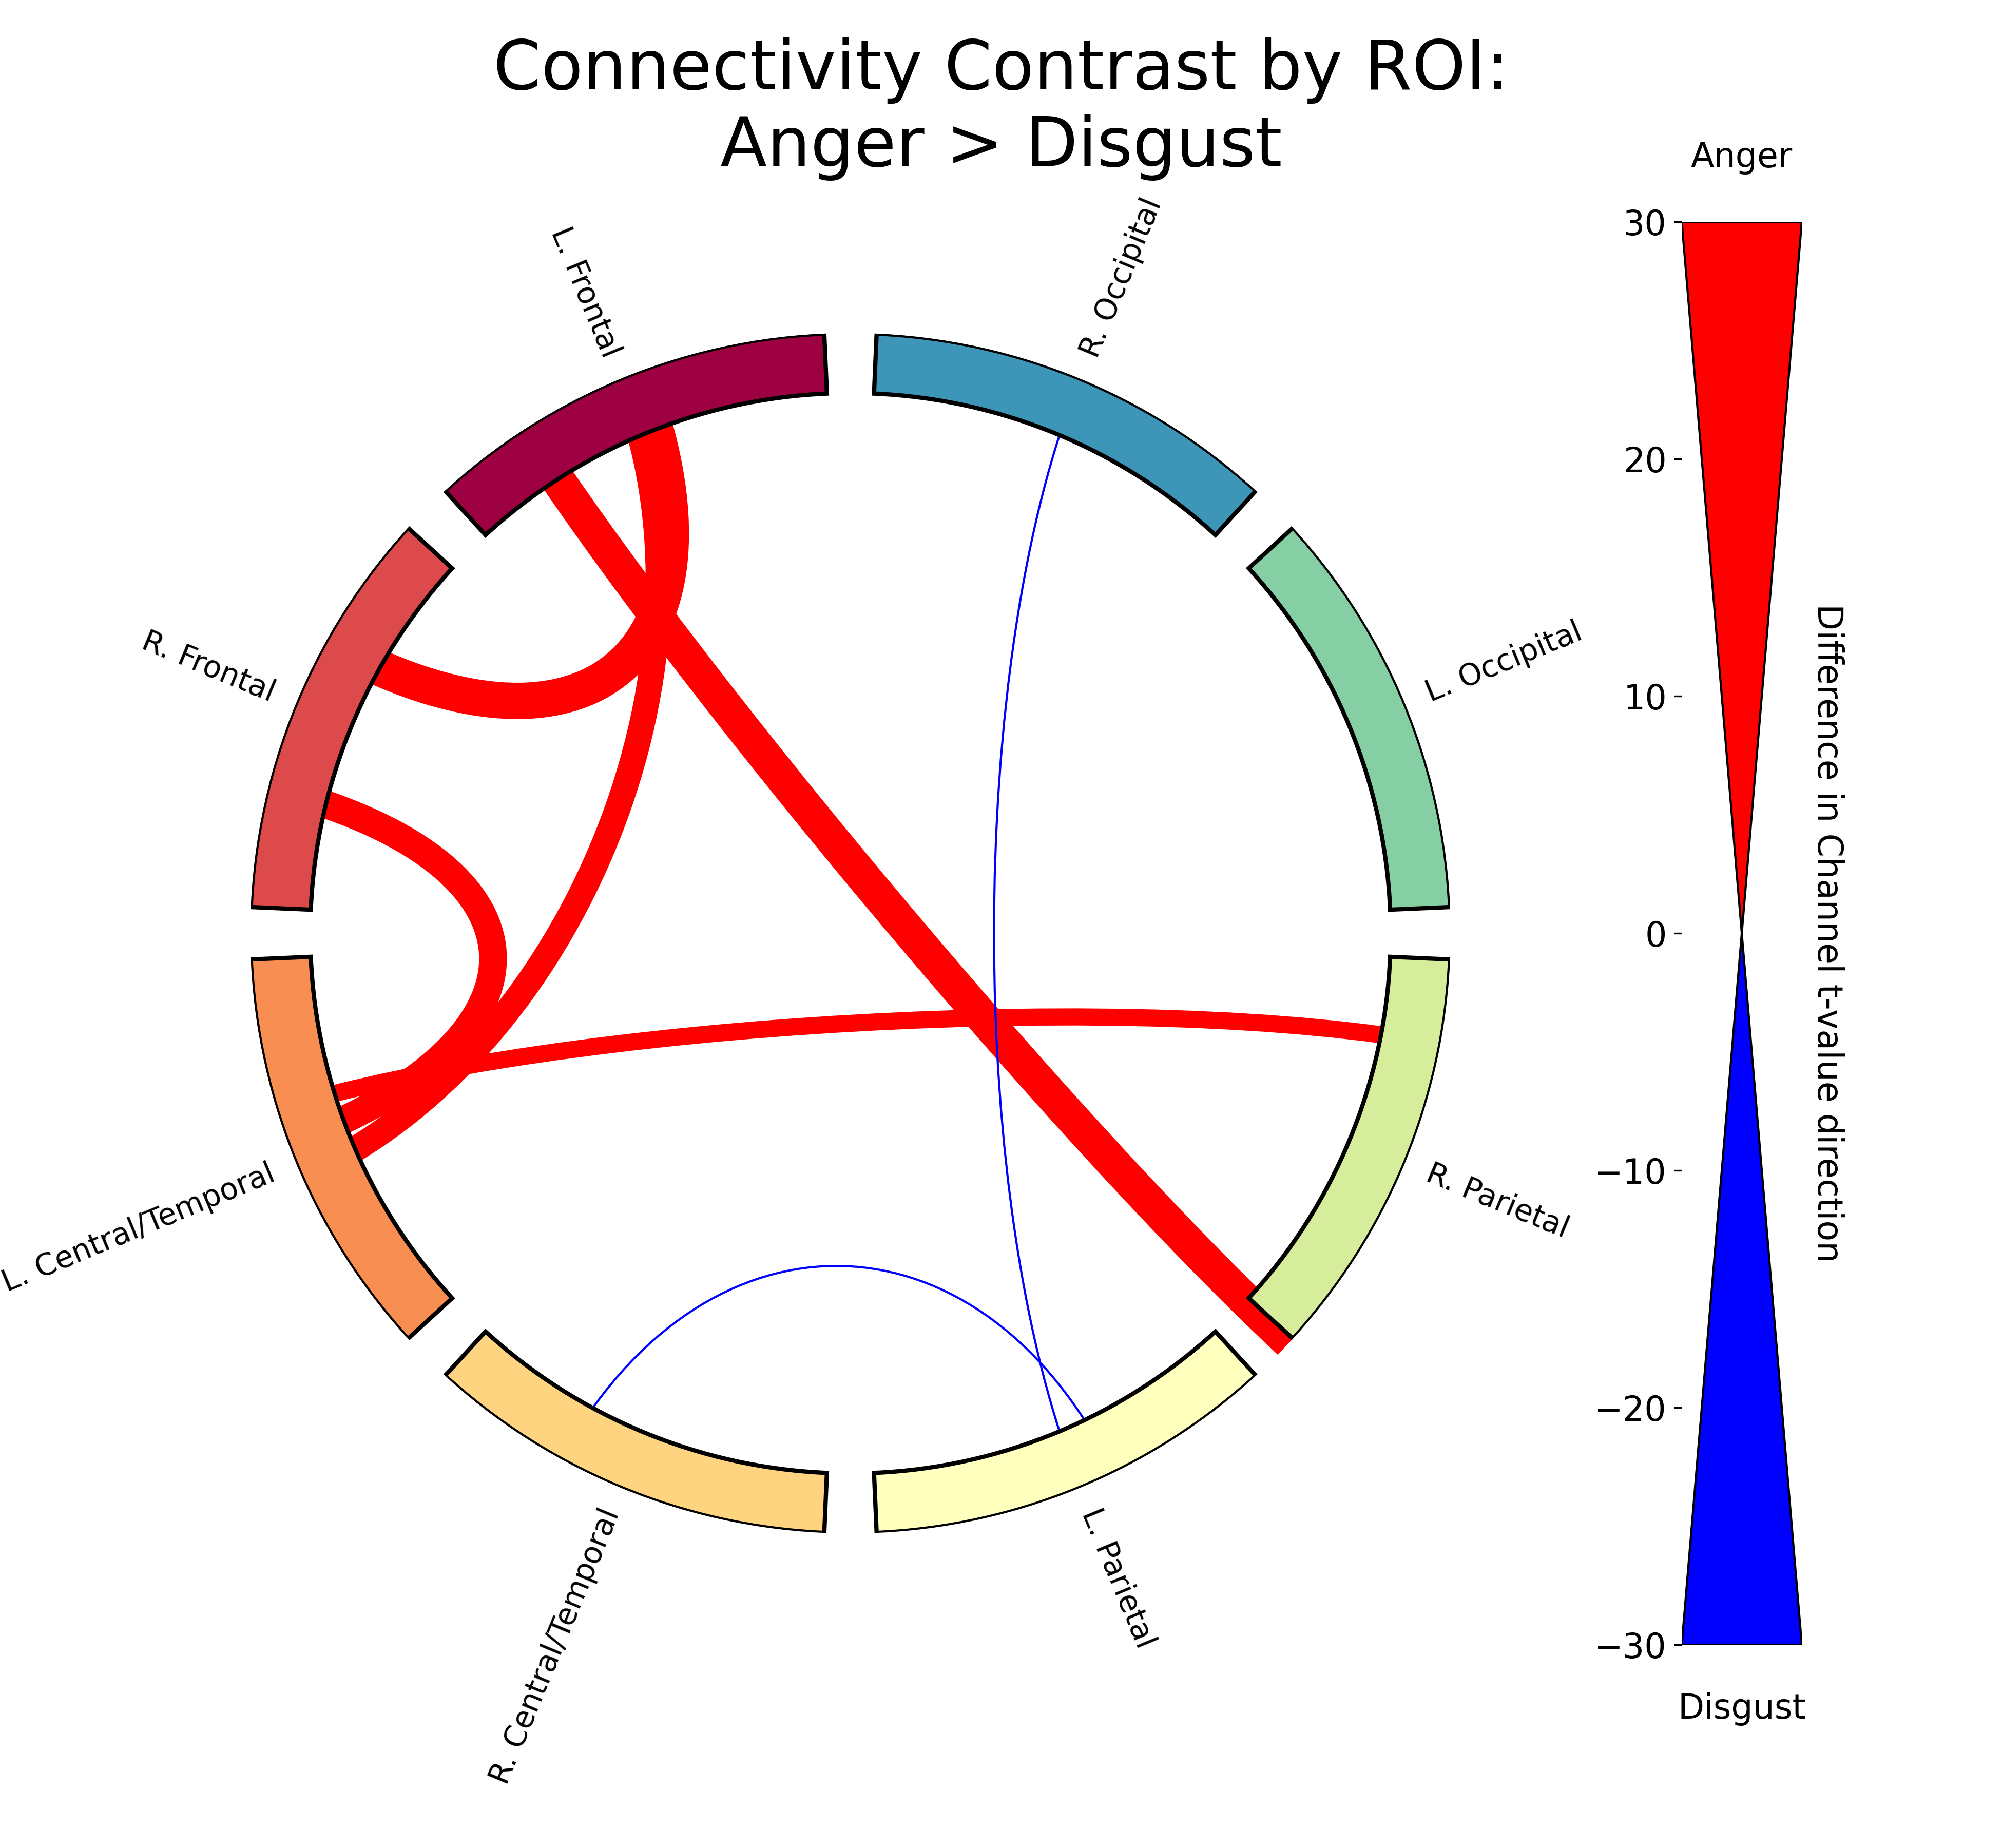
\includegraphics[width=0.45\textwidth]{C:/Users/super/OneDrive - Ontario Tech University/fNIRS_Emotions/plots/spectral_connectivity_time/chord_plots/group_level_t_tests_roi/emotion_Anger_Disgust.png}
    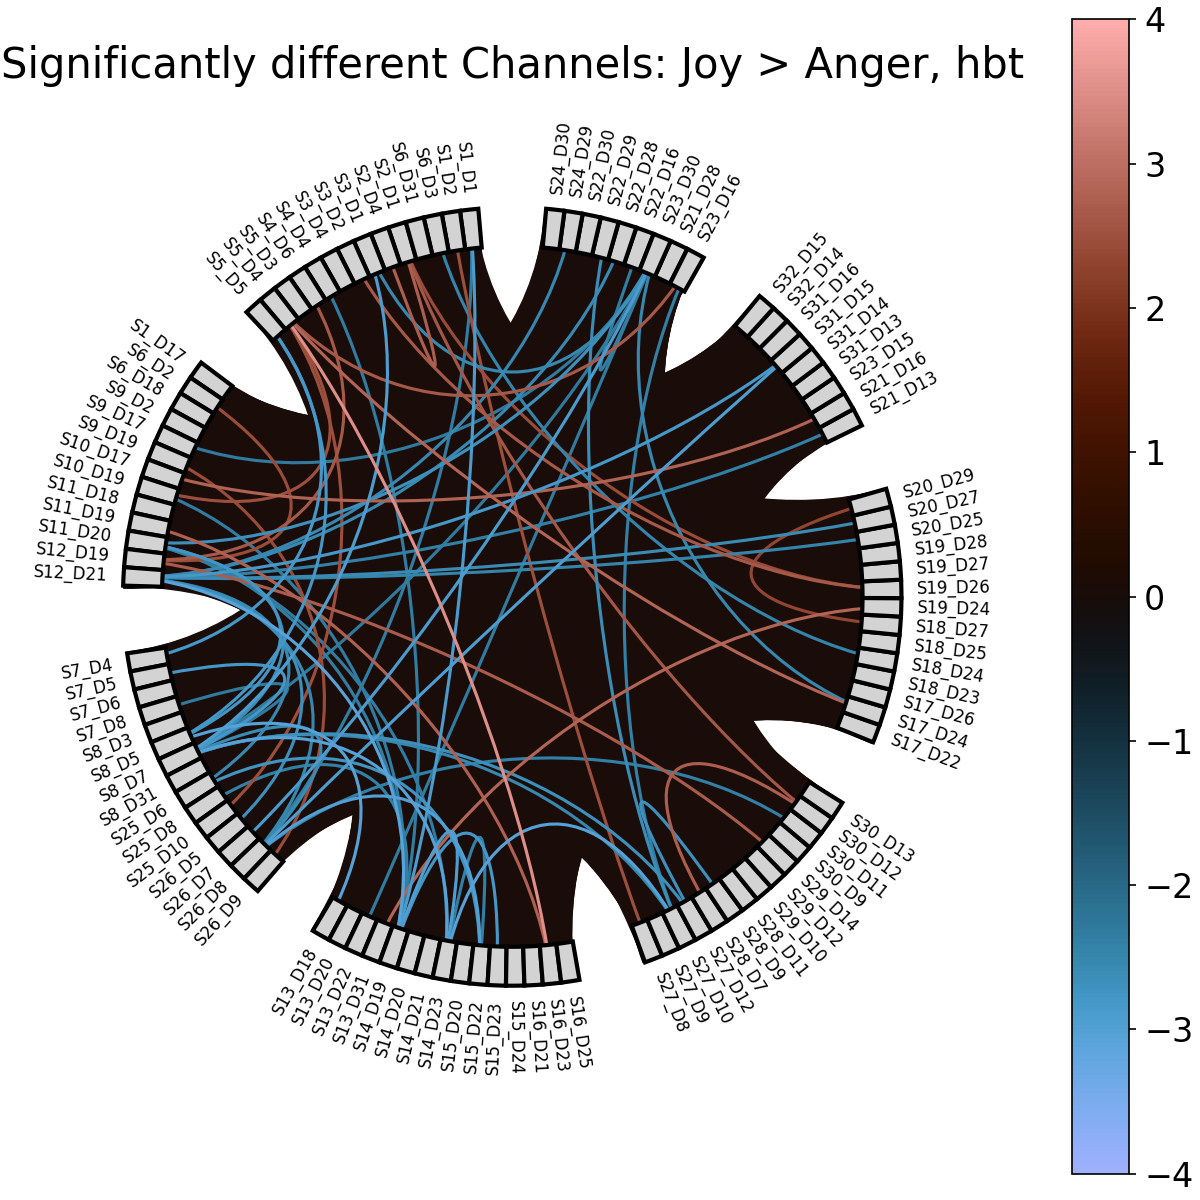
\includegraphics[width=0.45\textwidth]{C:/Users/super/OneDrive - Ontario Tech University/fNIRS_Emotions/plots/spectral_connectivity_time/chord_plots/group_level_t_tests_roi/emotion_Joy_Anger.png}
    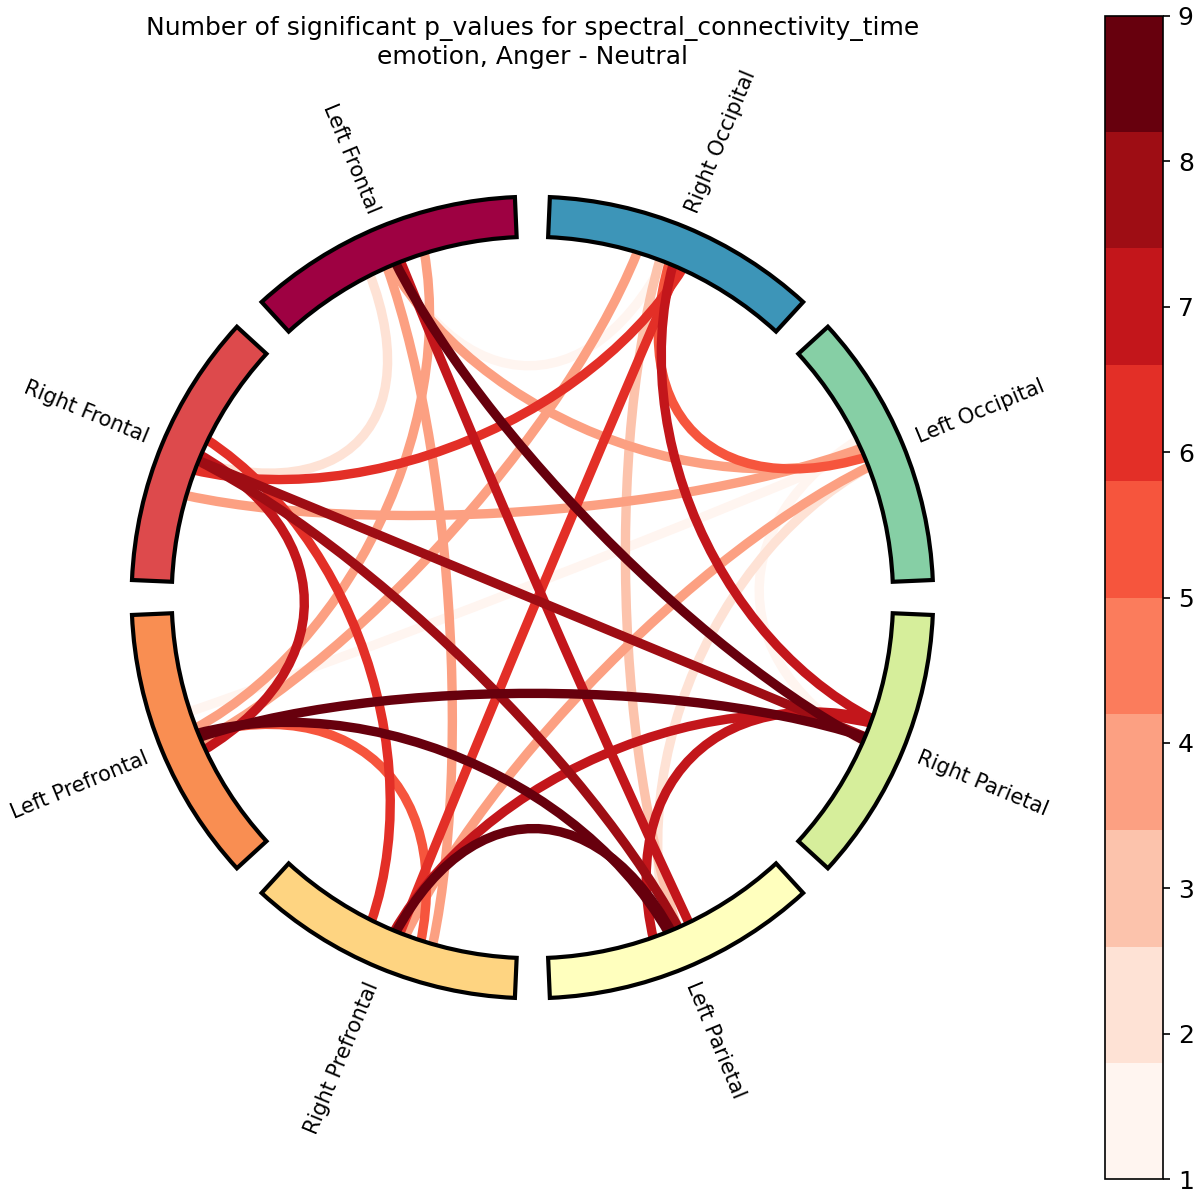
\includegraphics[width=0.45\textwidth]{C:/Users/super/OneDrive - Ontario Tech University/fNIRS_Emotions/plots/spectral_connectivity_time/chord_plots/group_level_t_tests_roi/emotion_Anger_Neutral.png}
    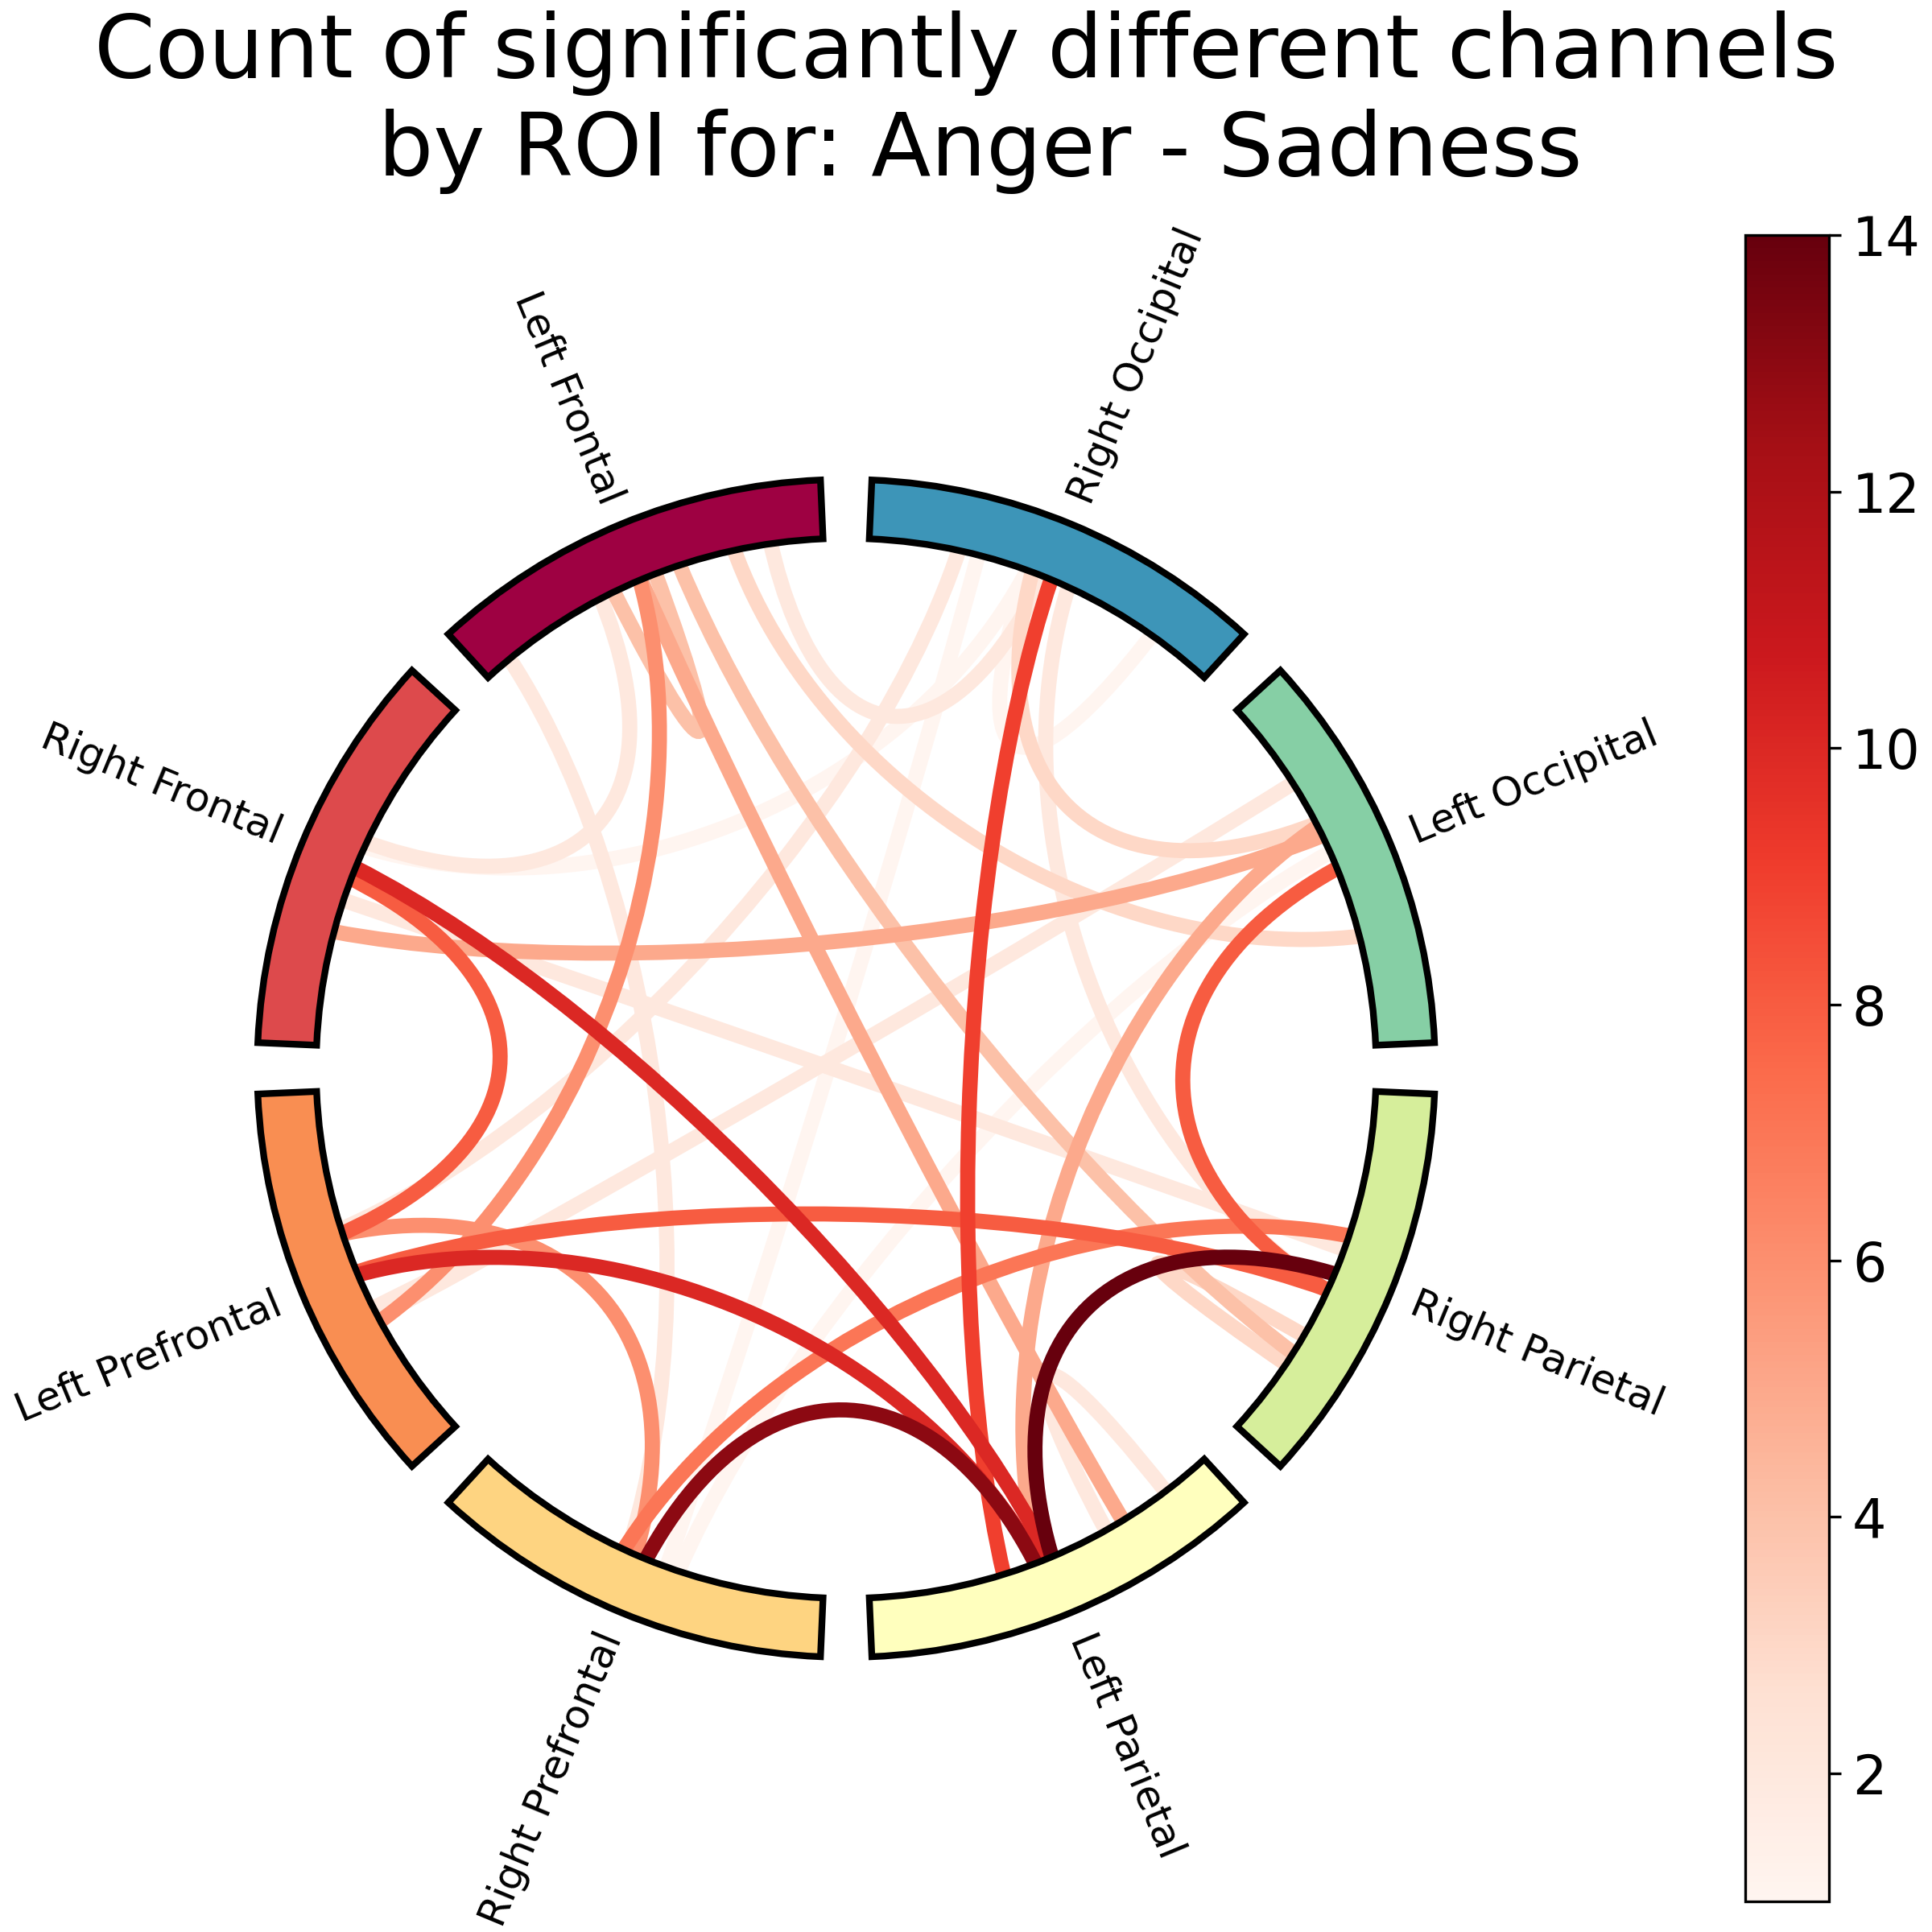
\includegraphics[width=0.45\textwidth]{C:/Users/super/OneDrive - Ontario Tech University/fNIRS_Emotions/plots/spectral_connectivity_time/chord_plots/group_level_t_tests_roi/emotion_Anger_Sadness.png}
    \caption[FC: Additional emotion contrasts]{Functional connectivity results for Anger contrasts: Anger vs. Disgust, Joy, Neutral, and Sadness. (1/4)}
    \label{fig:appendix_fc_emotion_analysis}
\end{figure}

\FloatBarrier

\begin{figure}[H]
    \ContinuedFloat
    \centering
    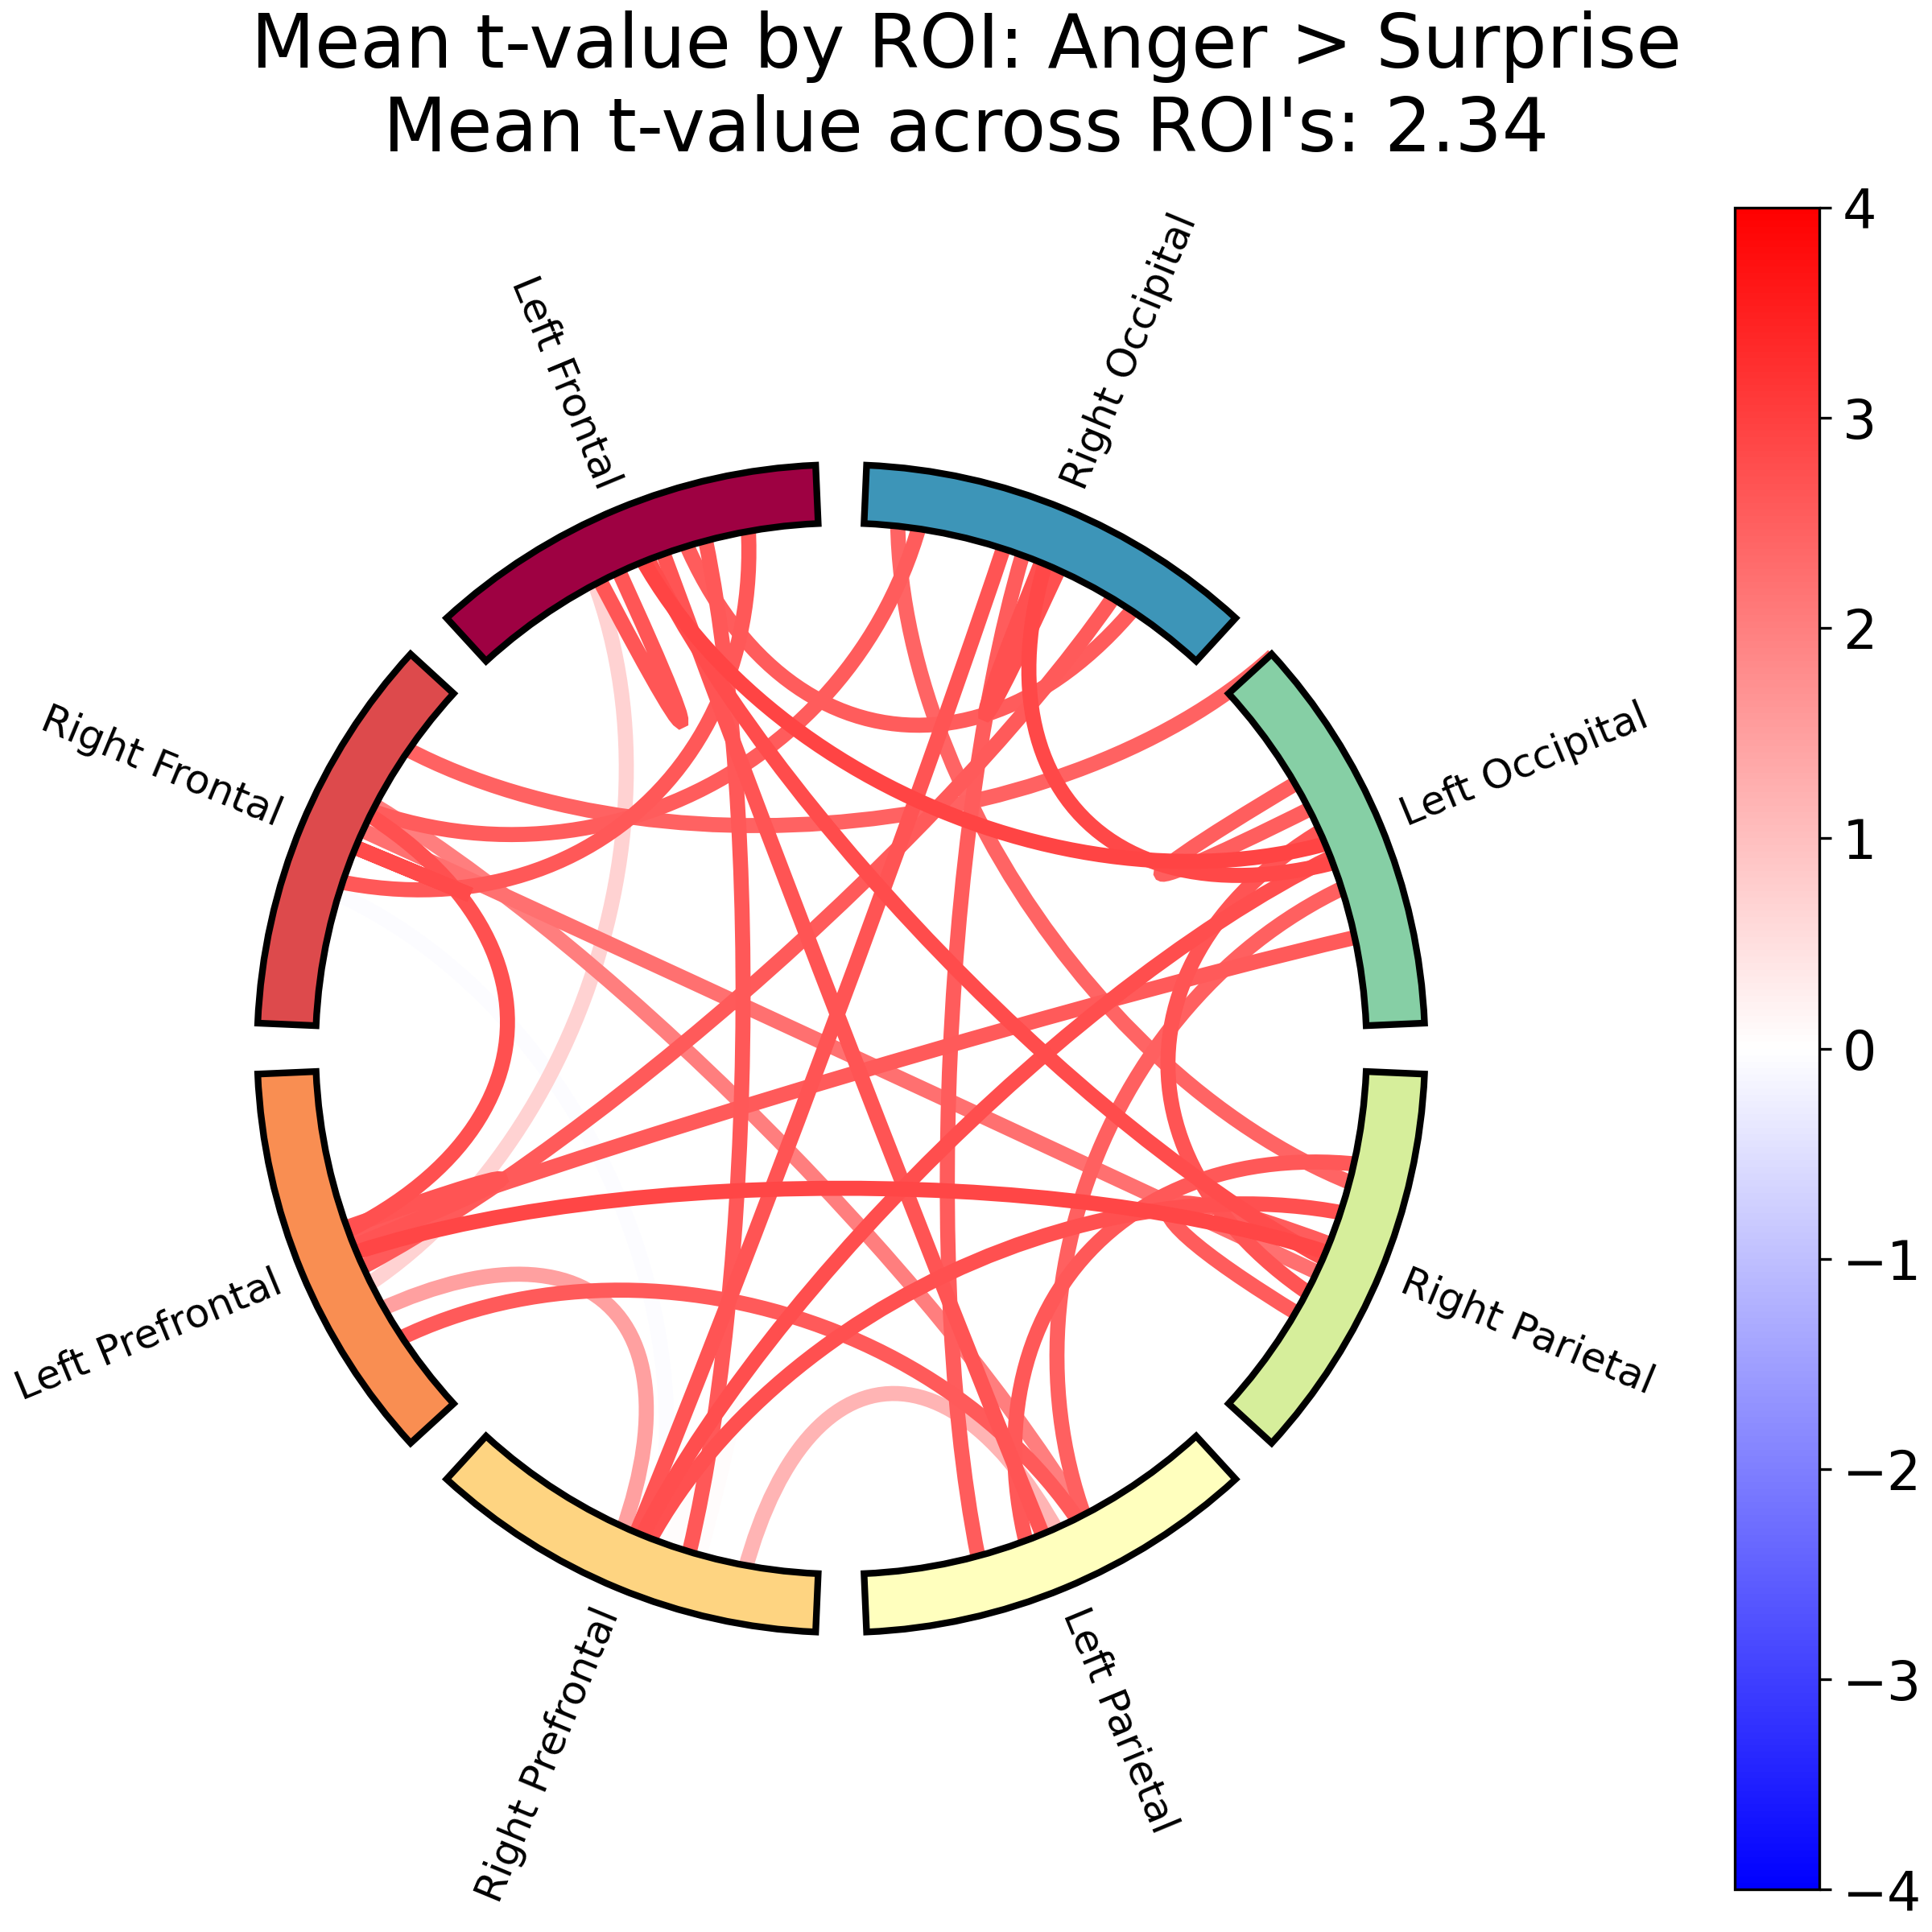
\includegraphics[width=0.49\textwidth]{C:/Users/super/OneDrive - Ontario Tech University/fNIRS_Emotions/plots/spectral_connectivity_time/chord_plots/group_level_t_tests_roi/emotion_Anger_Surprise.png}
    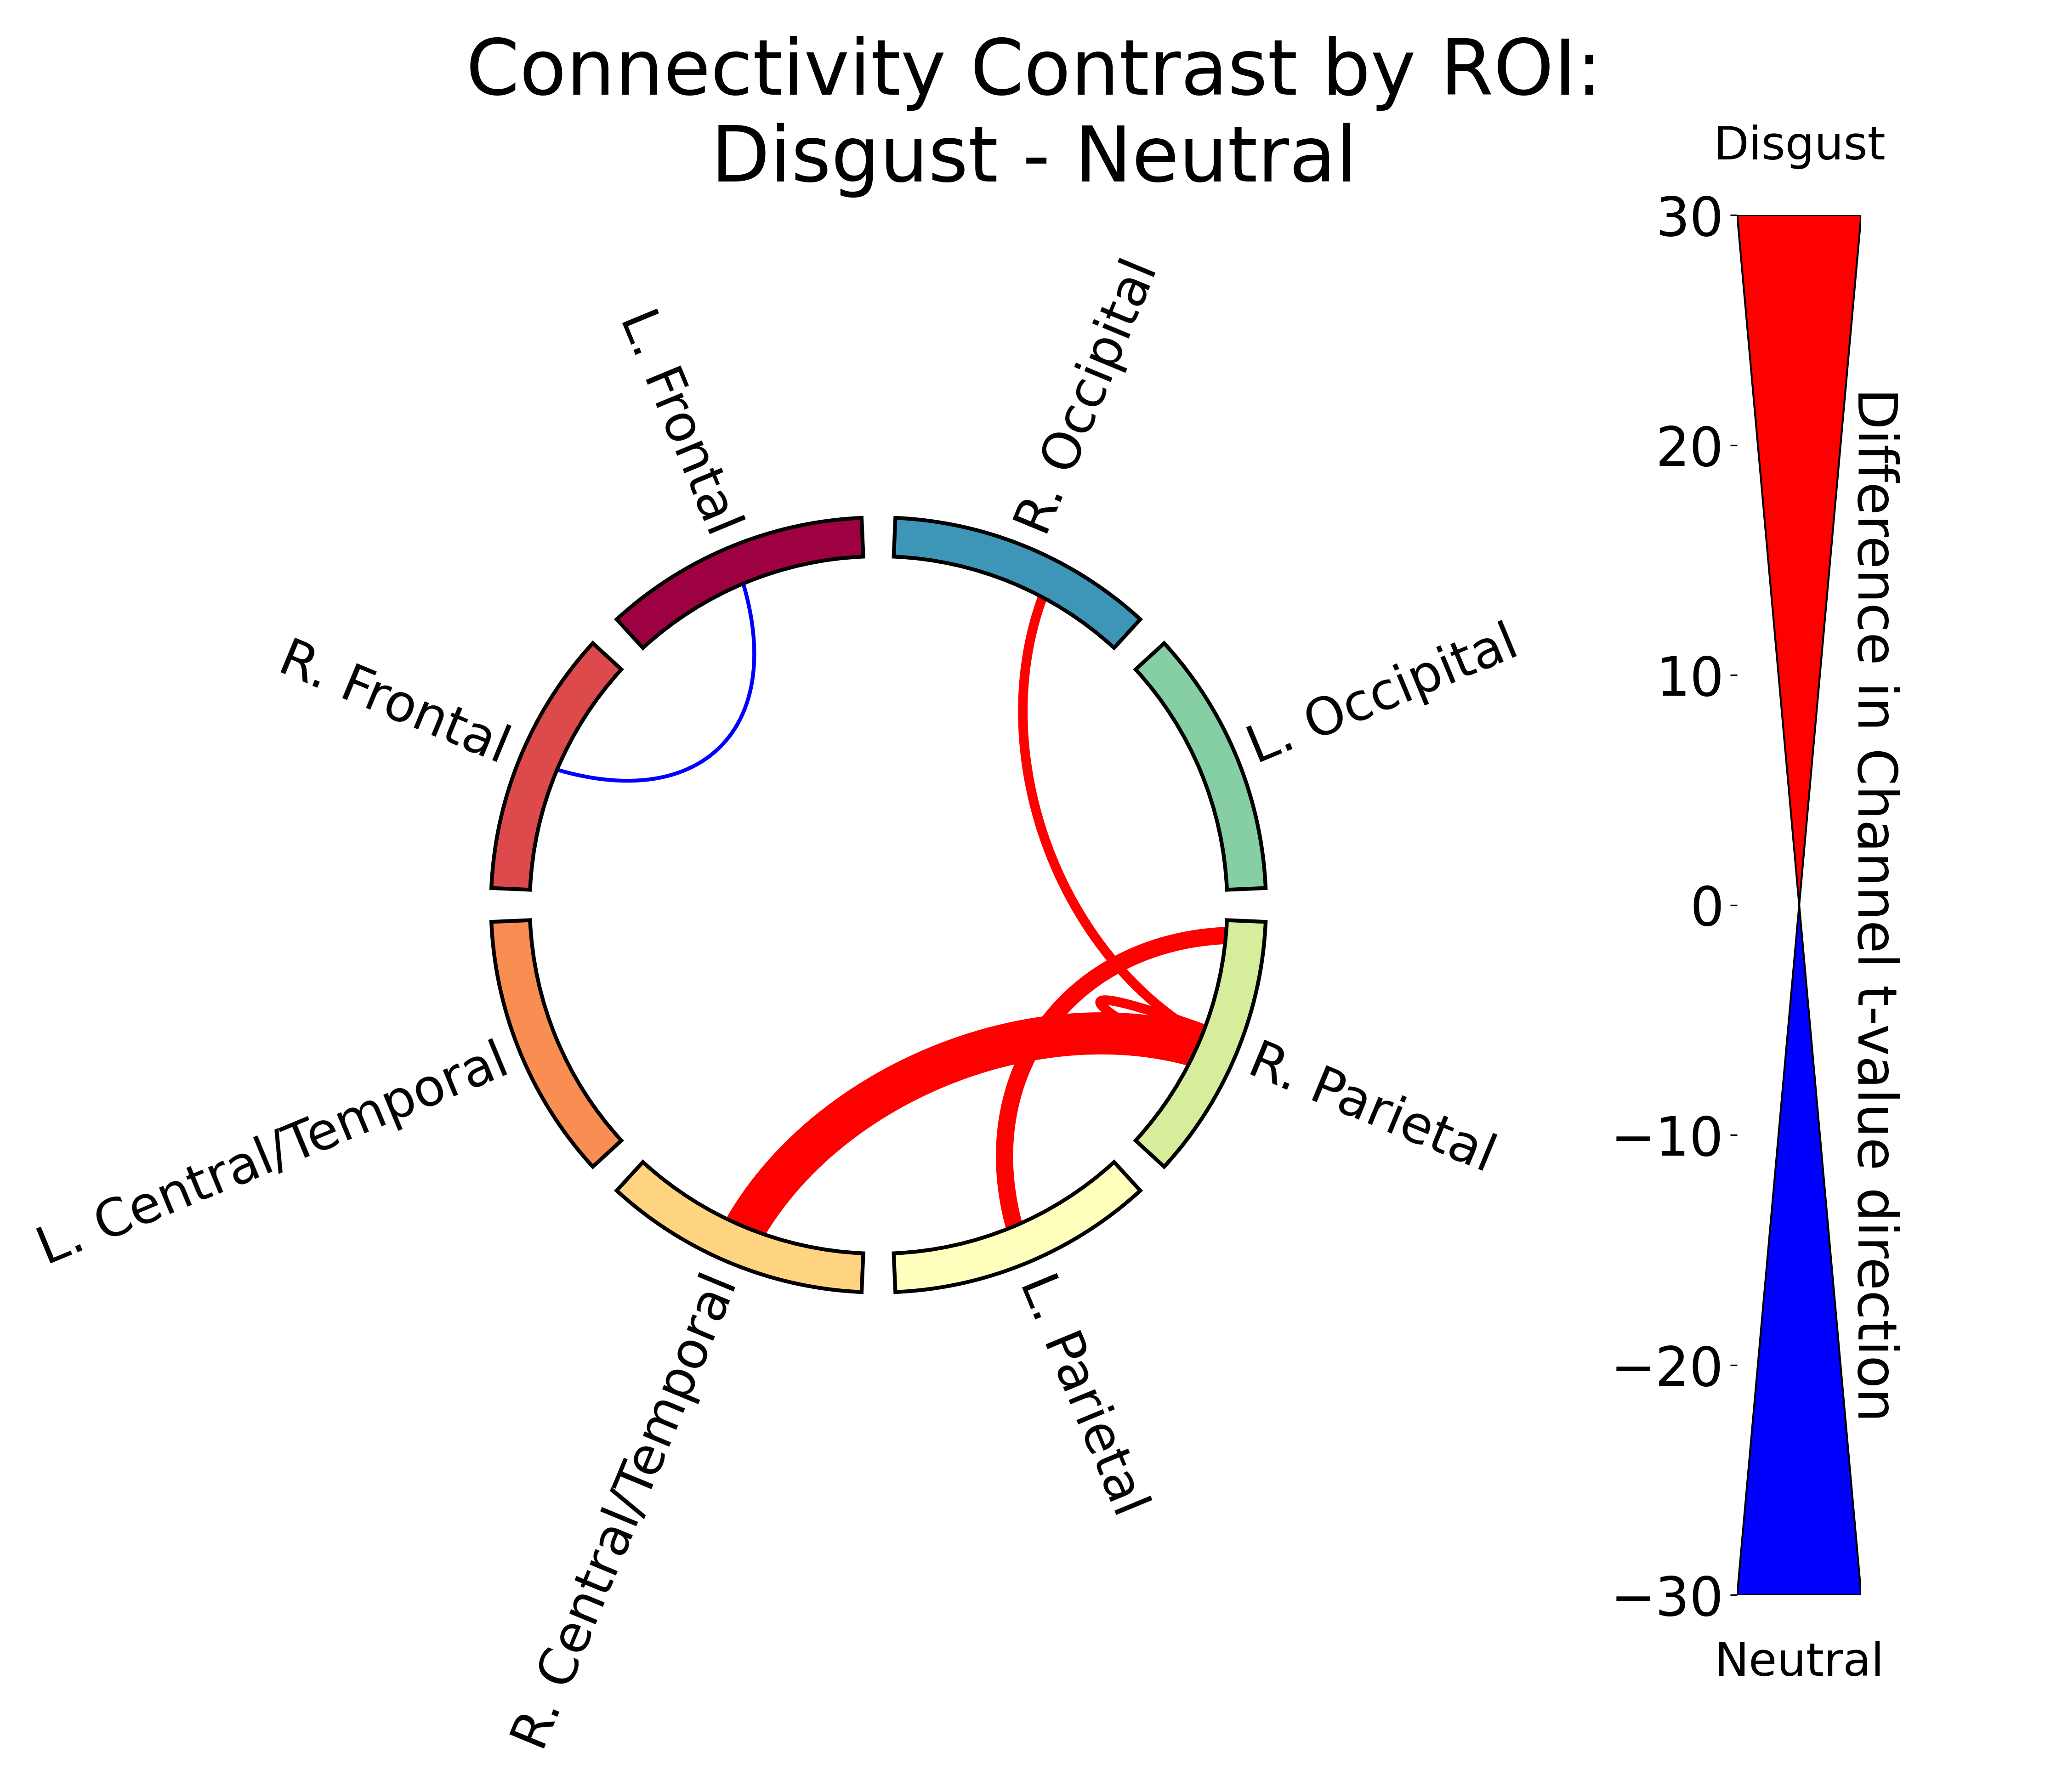
\includegraphics[width=0.49\textwidth]{C:/Users/super/OneDrive - Ontario Tech University/fNIRS_Emotions/plots/spectral_connectivity_time/chord_plots/group_level_t_tests_roi/emotion_Disgust_Neutral.png}
    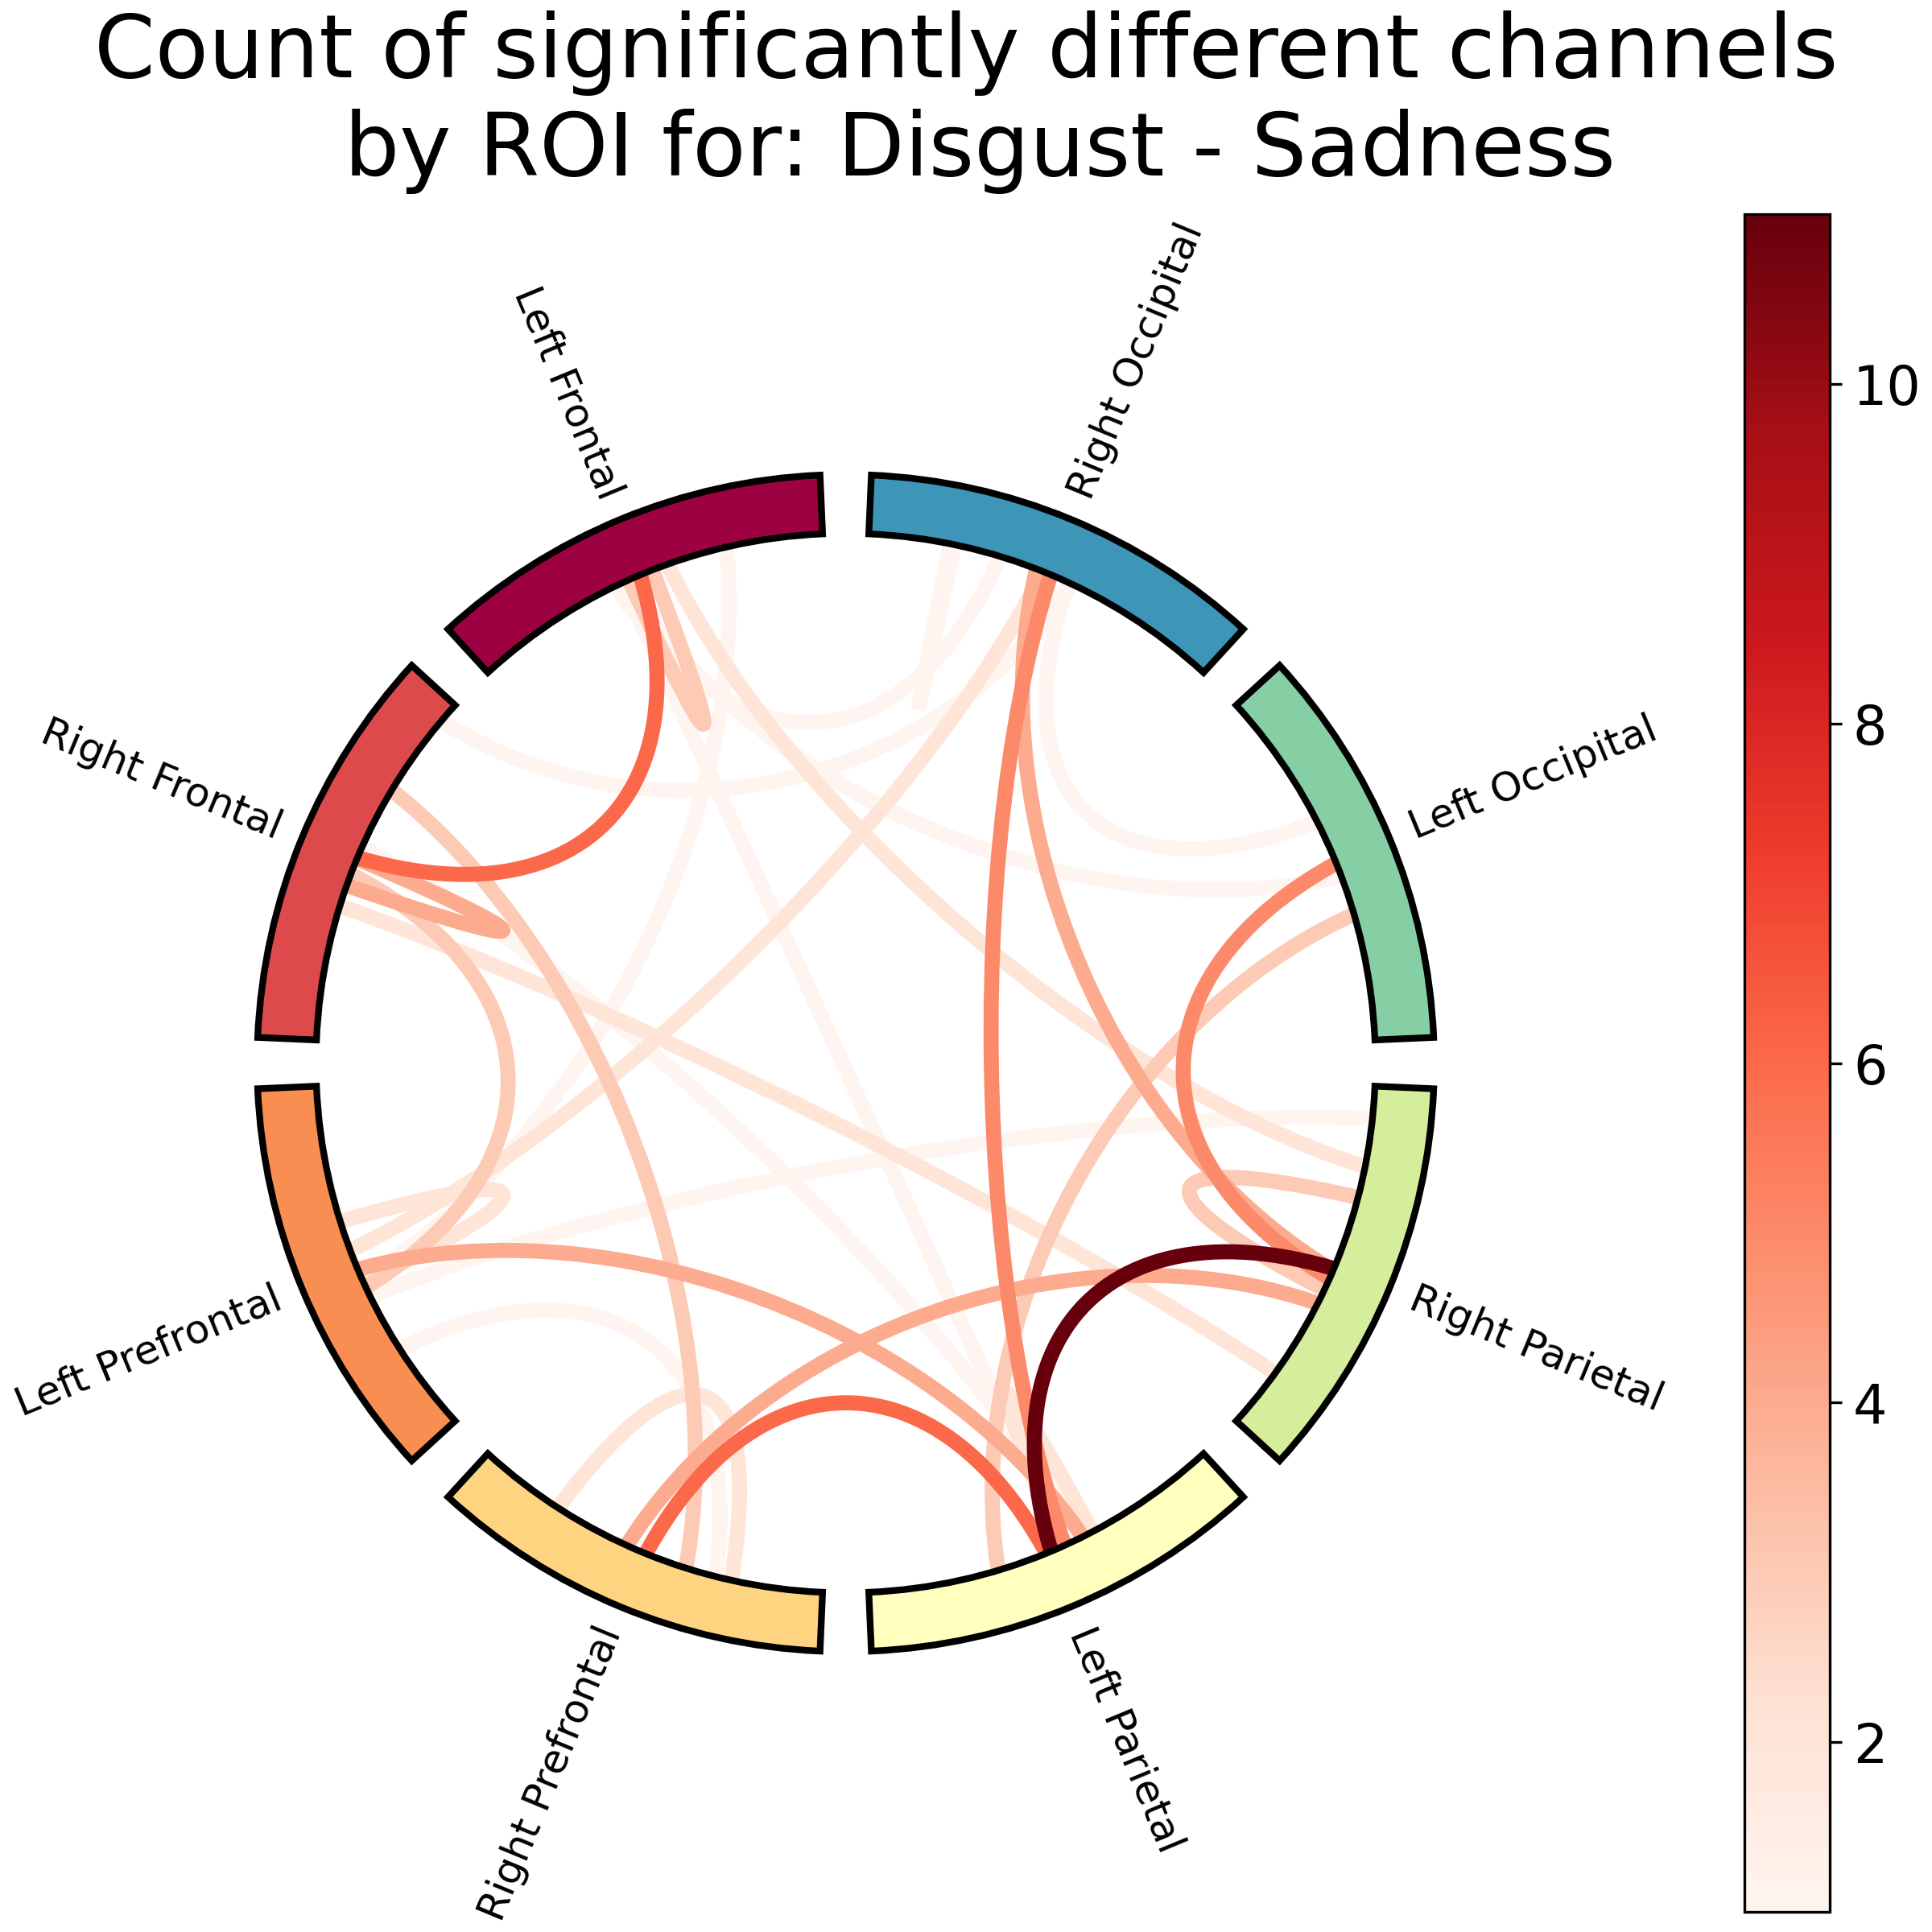
\includegraphics[width=0.49\textwidth]{C:/Users/super/OneDrive - Ontario Tech University/fNIRS_Emotions/plots/spectral_connectivity_time/chord_plots/group_level_t_tests_roi/emotion_Disgust_Sadness.png}
    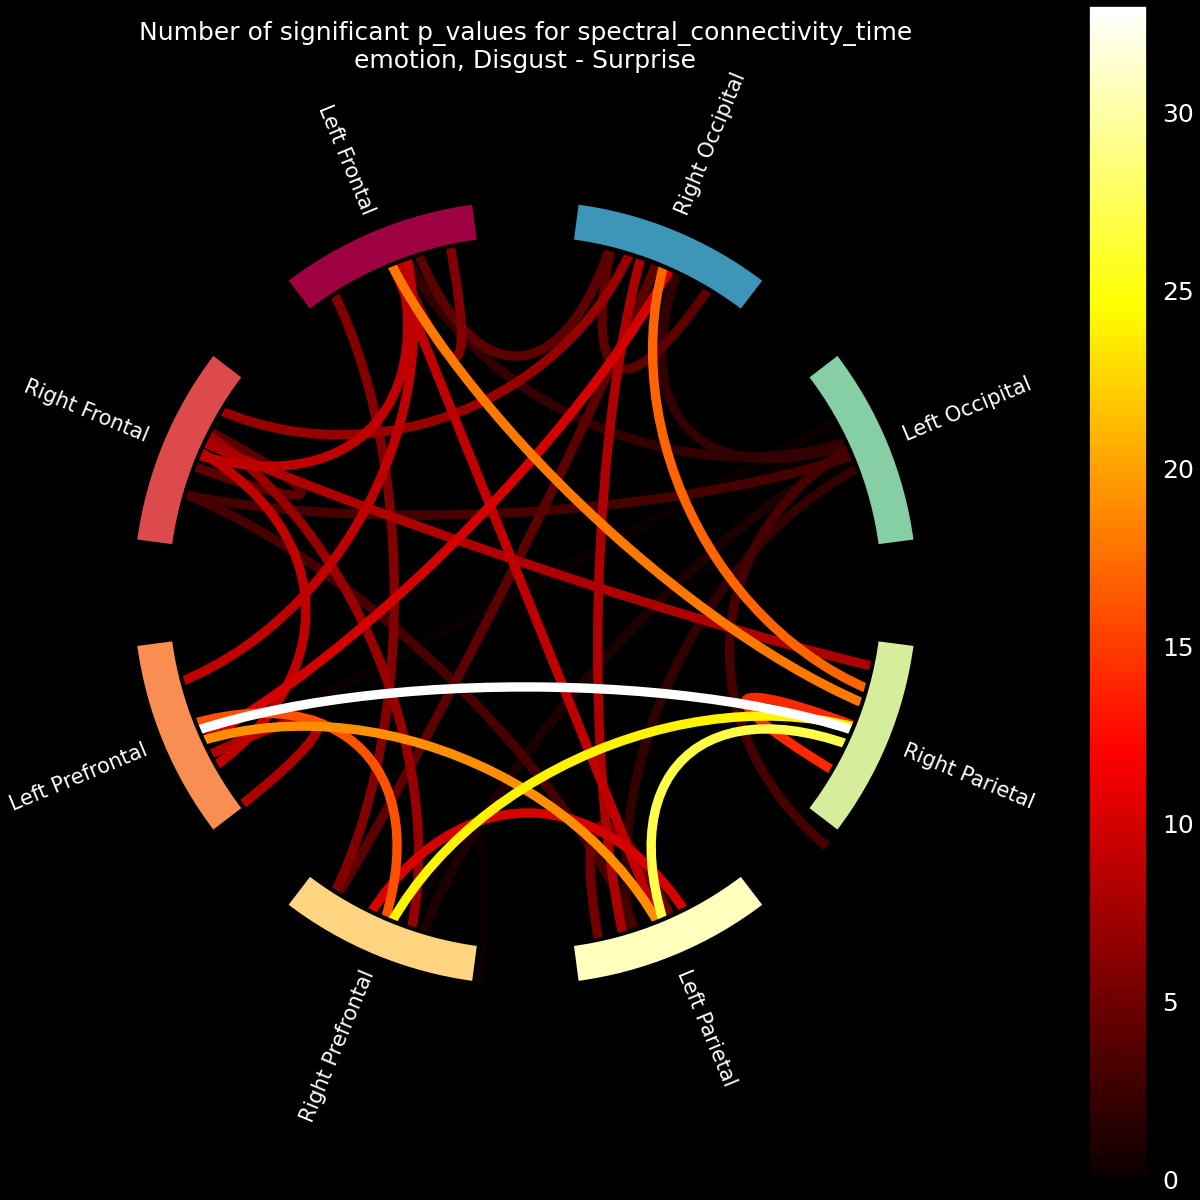
\includegraphics[width=0.49\textwidth]{C:/Users/super/OneDrive - Ontario Tech University/fNIRS_Emotions/plots/spectral_connectivity_time/chord_plots/group_level_t_tests_roi/emotion_Disgust_Surprise.png}
    \caption*{Functional connectivity results for Anger vs. Surprise and Disgust contrasts: Disgust vs. Neutral, Sadness, and Surprise. (2/4)}
\end{figure}

\FloatBarrier

\begin{figure}[H]
    \ContinuedFloat
    \centering
    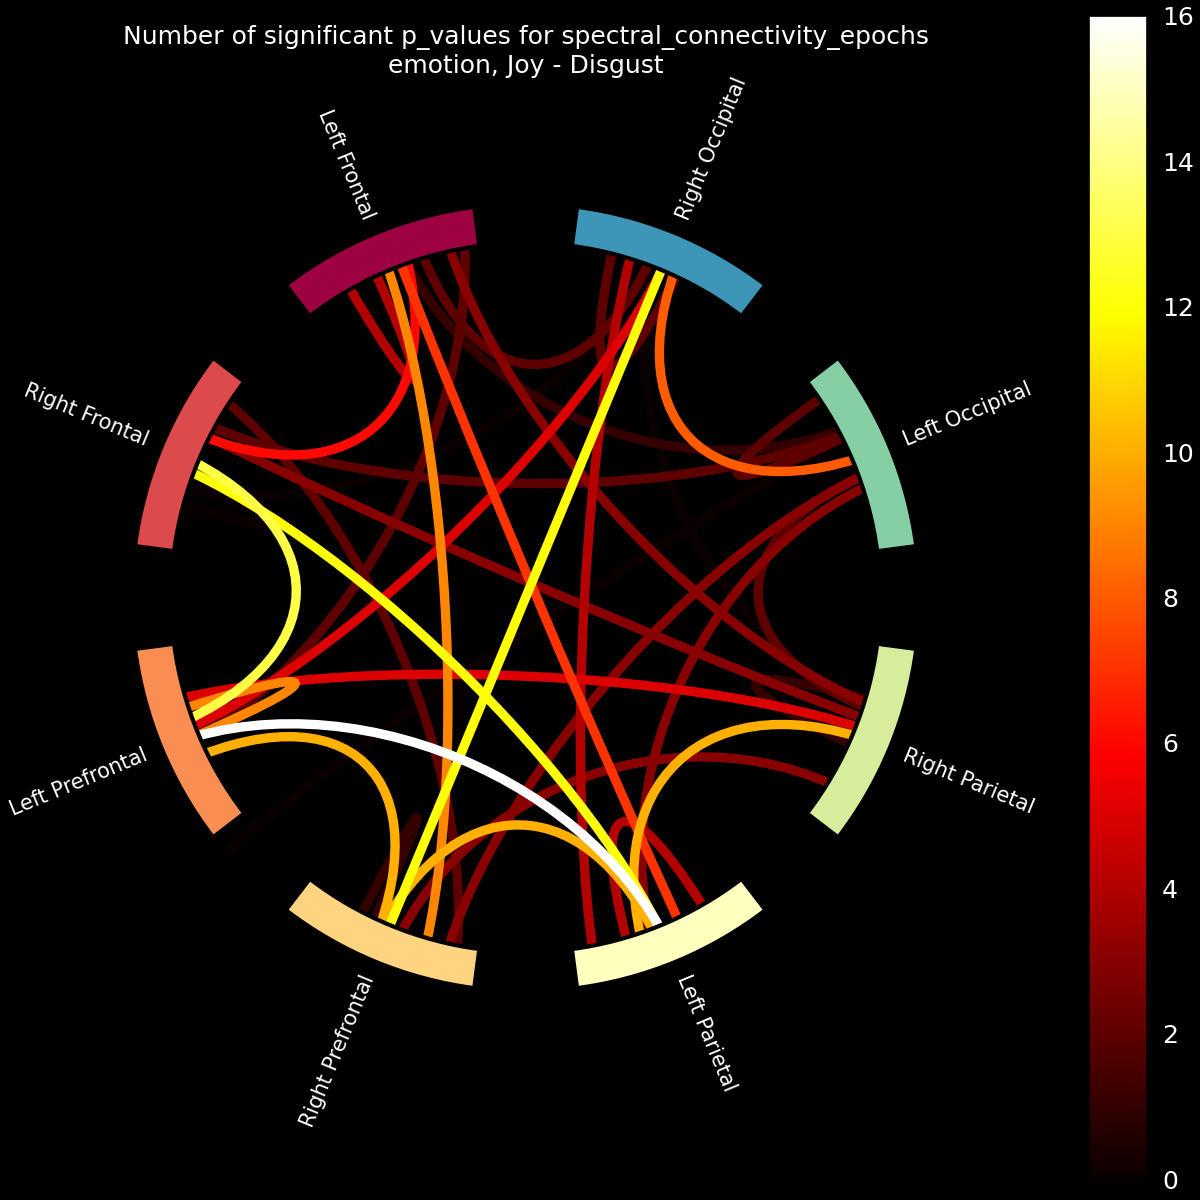
\includegraphics[width=0.49\textwidth]{C:/Users/super/OneDrive - Ontario Tech University/fNIRS_Emotions/plots/spectral_connectivity_time/chord_plots/group_level_t_tests_roi/emotion_Joy_Disgust.png}
    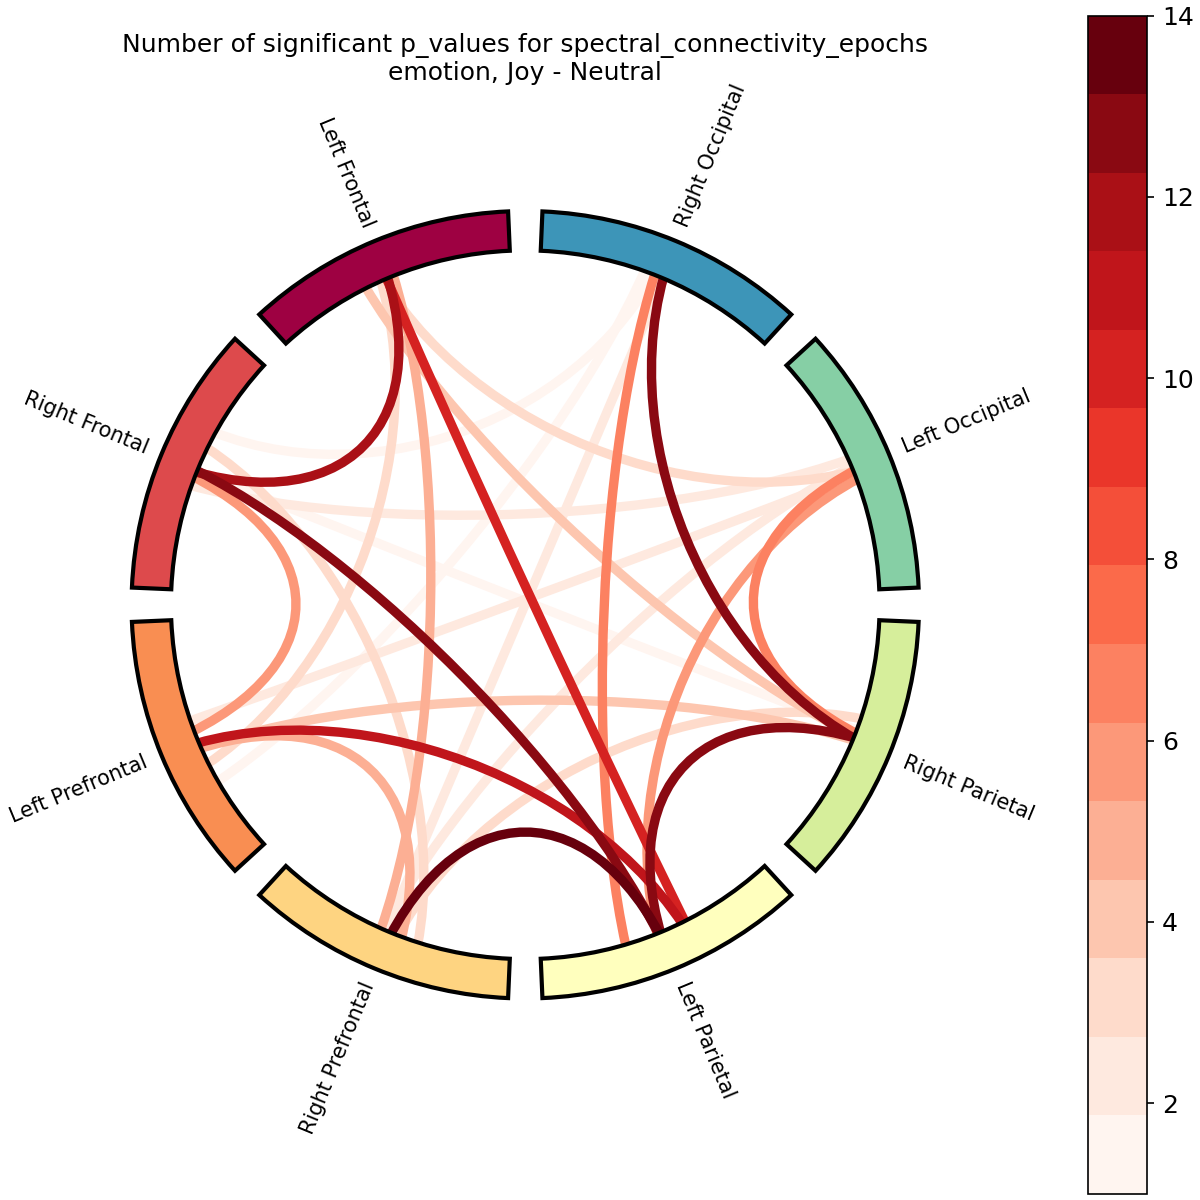
\includegraphics[width=0.49\textwidth]{C:/Users/super/OneDrive - Ontario Tech University/fNIRS_Emotions/plots/spectral_connectivity_time/chord_plots/group_level_t_tests_roi/emotion_Joy_Neutral.png}
    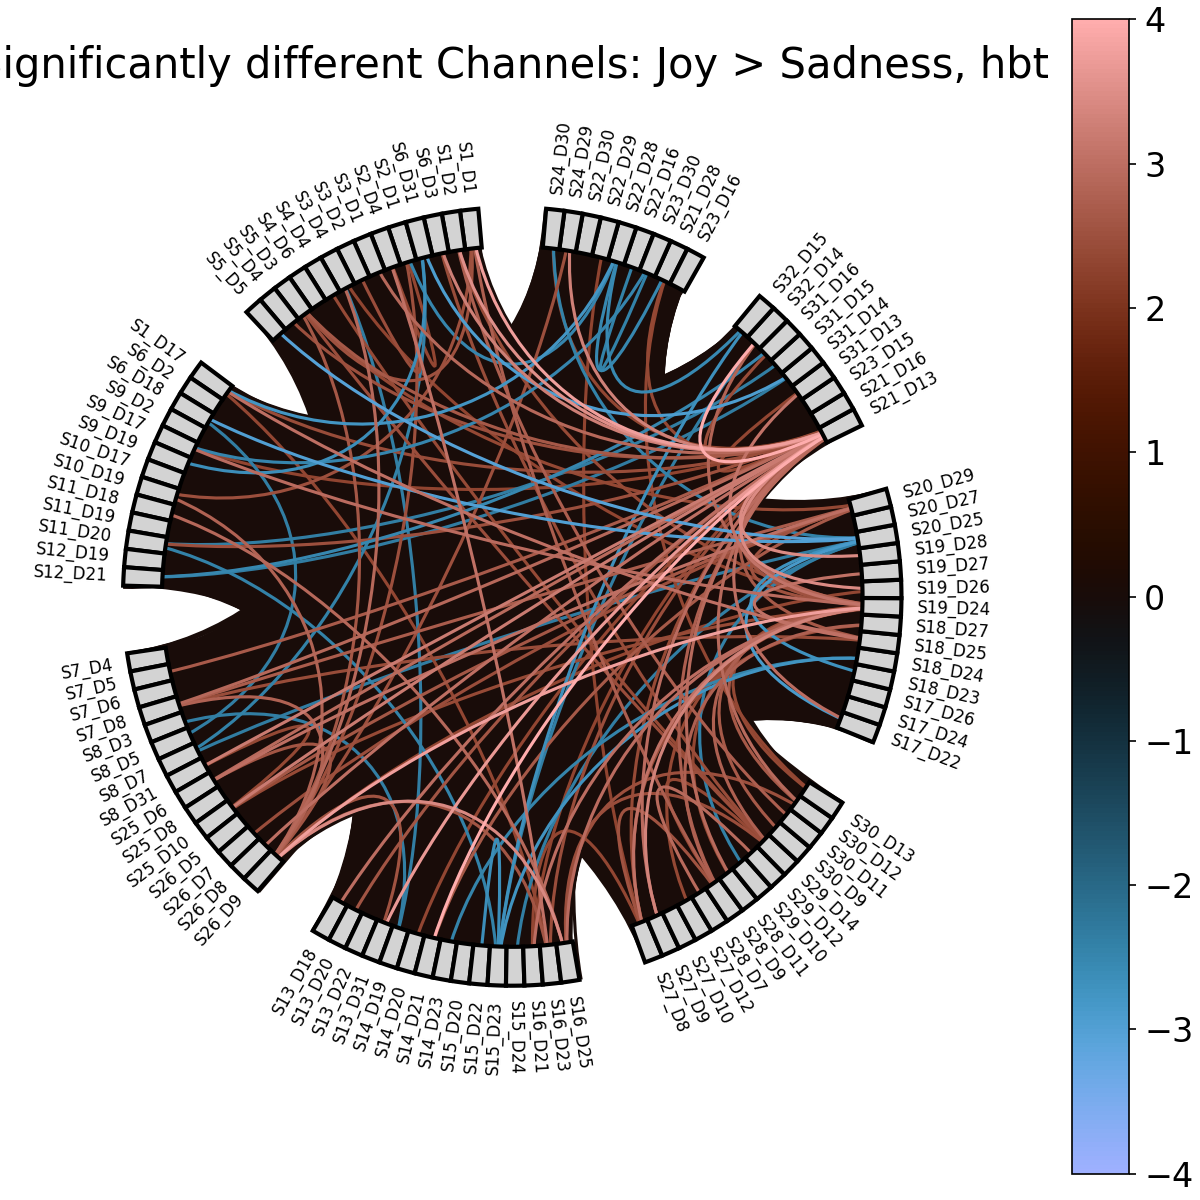
\includegraphics[width=0.49\textwidth]{C:/Users/super/OneDrive - Ontario Tech University/fNIRS_Emotions/plots/spectral_connectivity_time/chord_plots/group_level_t_tests_roi/emotion_Joy_Sadness.png}
    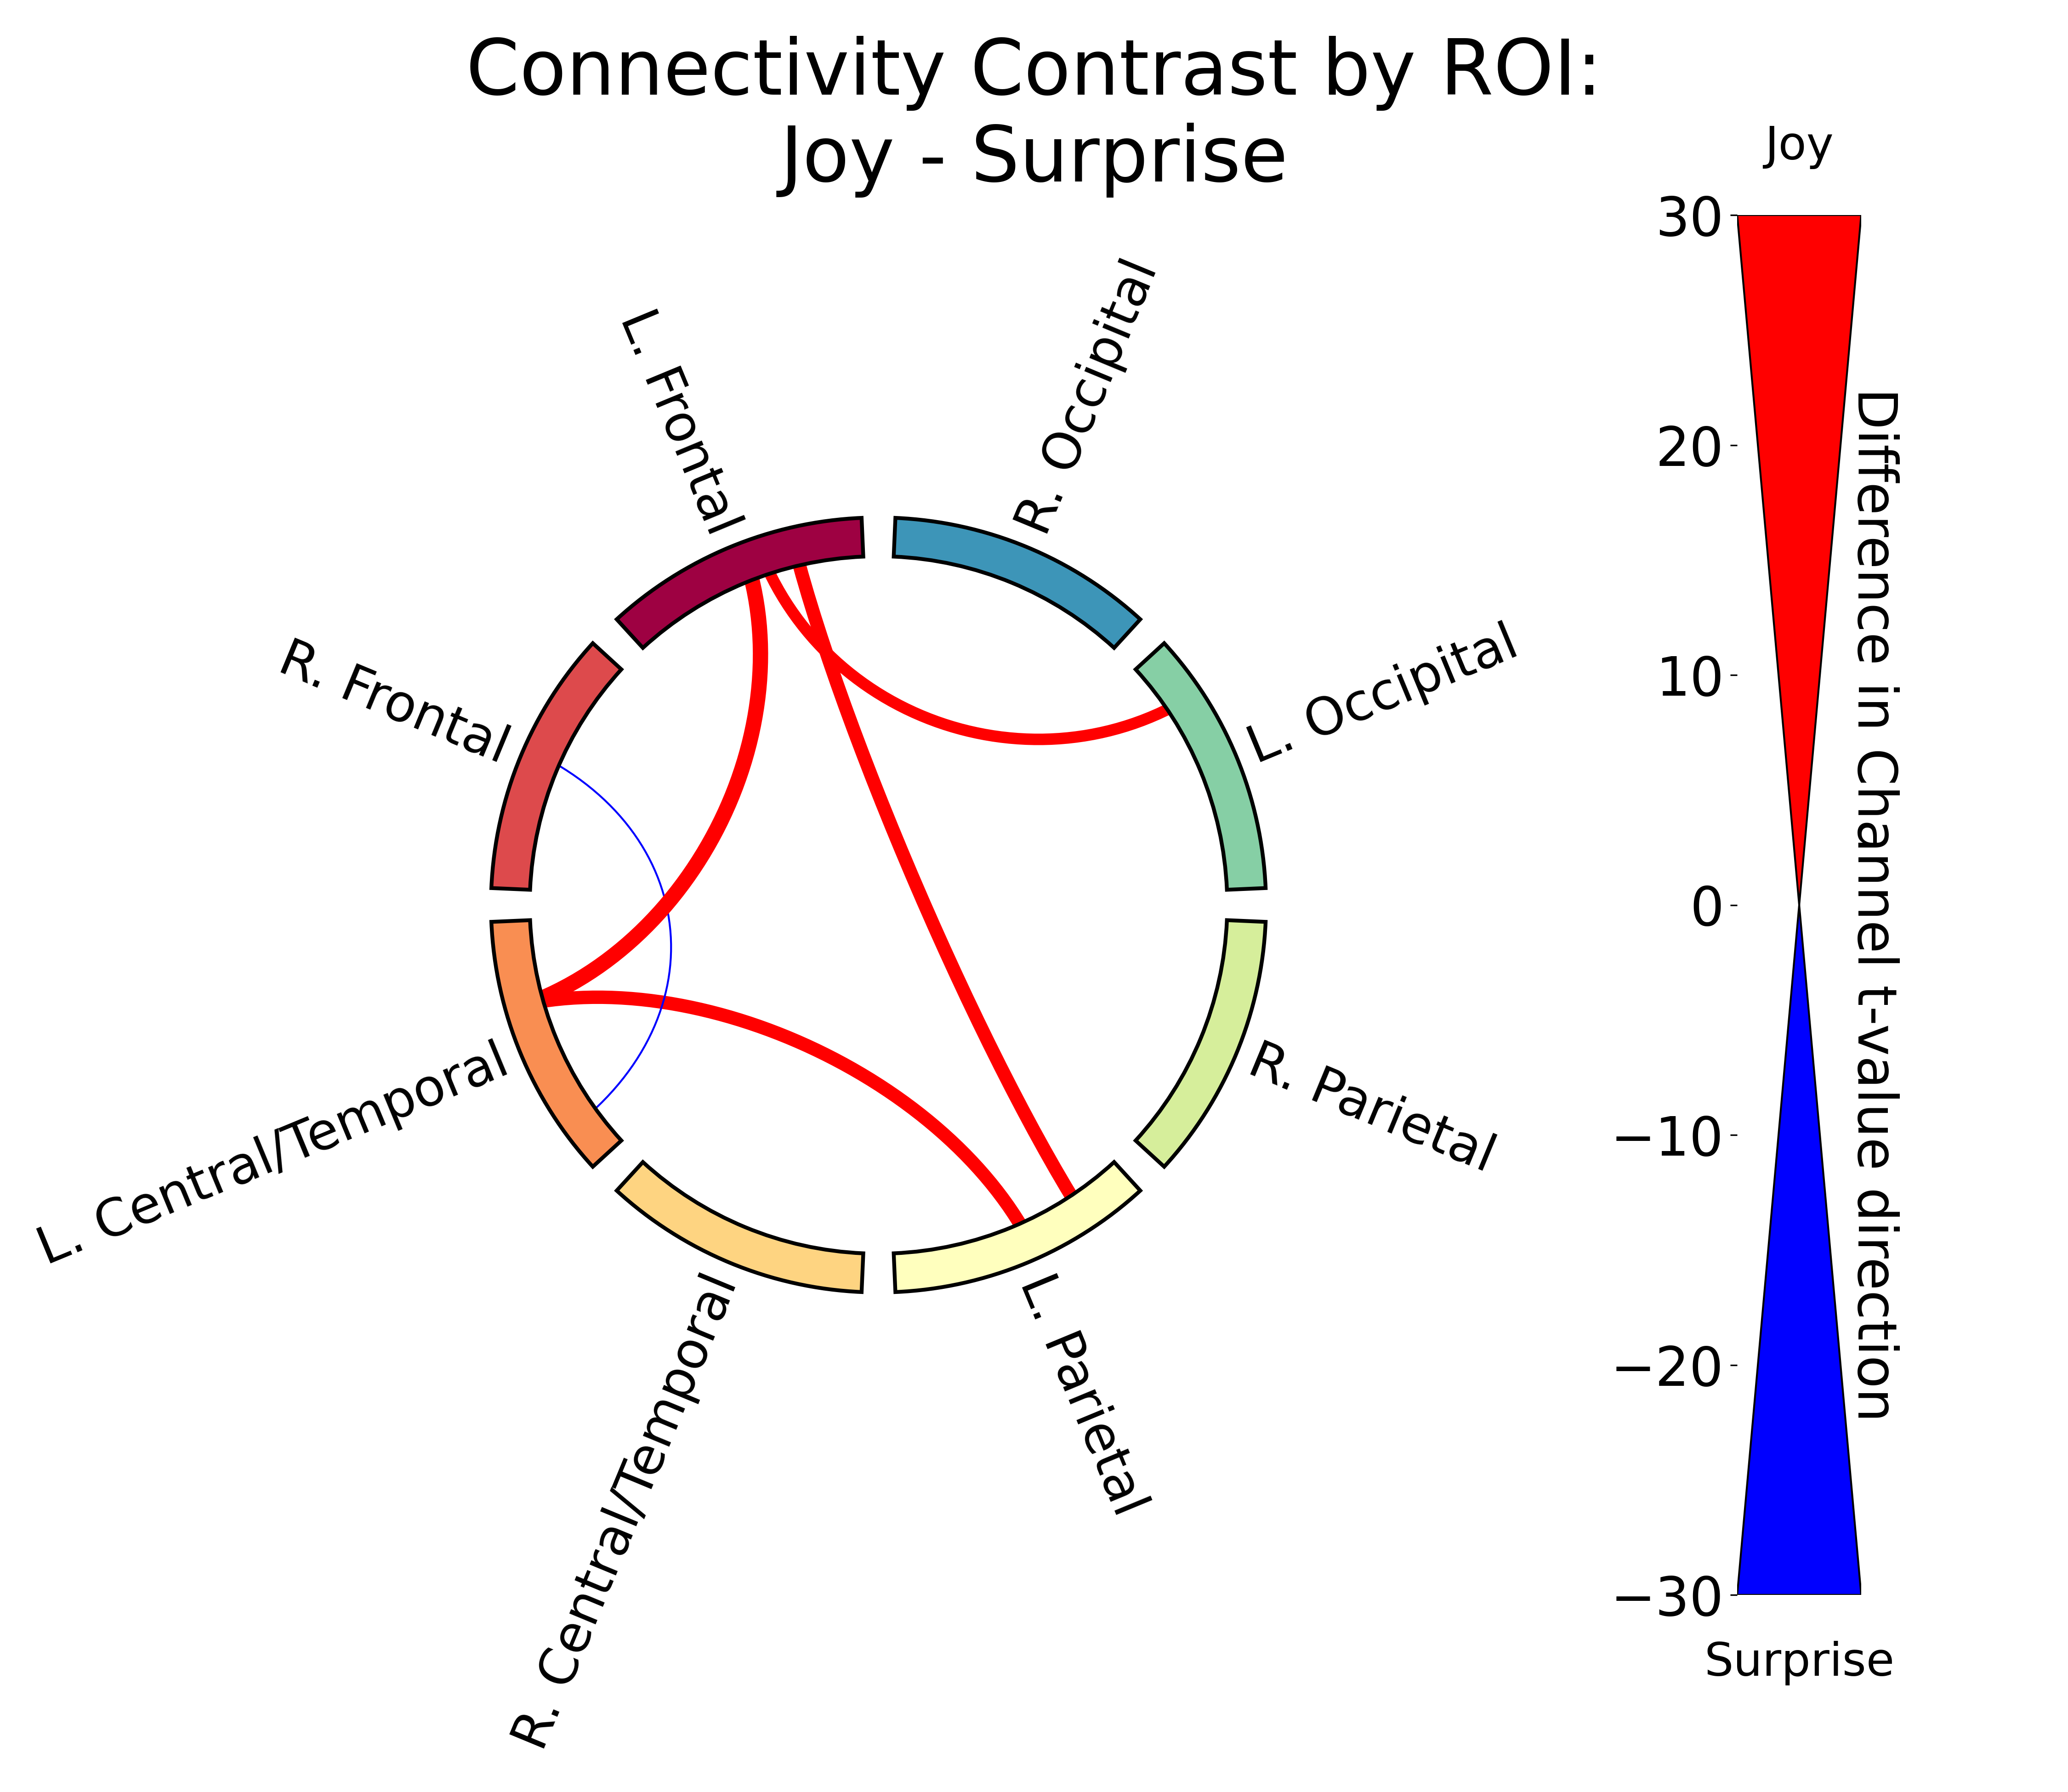
\includegraphics[width=0.49\textwidth]{C:/Users/super/OneDrive - Ontario Tech University/fNIRS_Emotions/plots/spectral_connectivity_time/chord_plots/group_level_t_tests_roi/emotion_Joy_Surprise.png}
    \caption*{Functional connectivity results for Joy contrasts: Joy vs. Disgust, Neutral, Sadness, and Surprise. (3/4)}
\end{figure}

\FloatBarrier

\begin{figure}[H]
    \ContinuedFloat
    \centering
    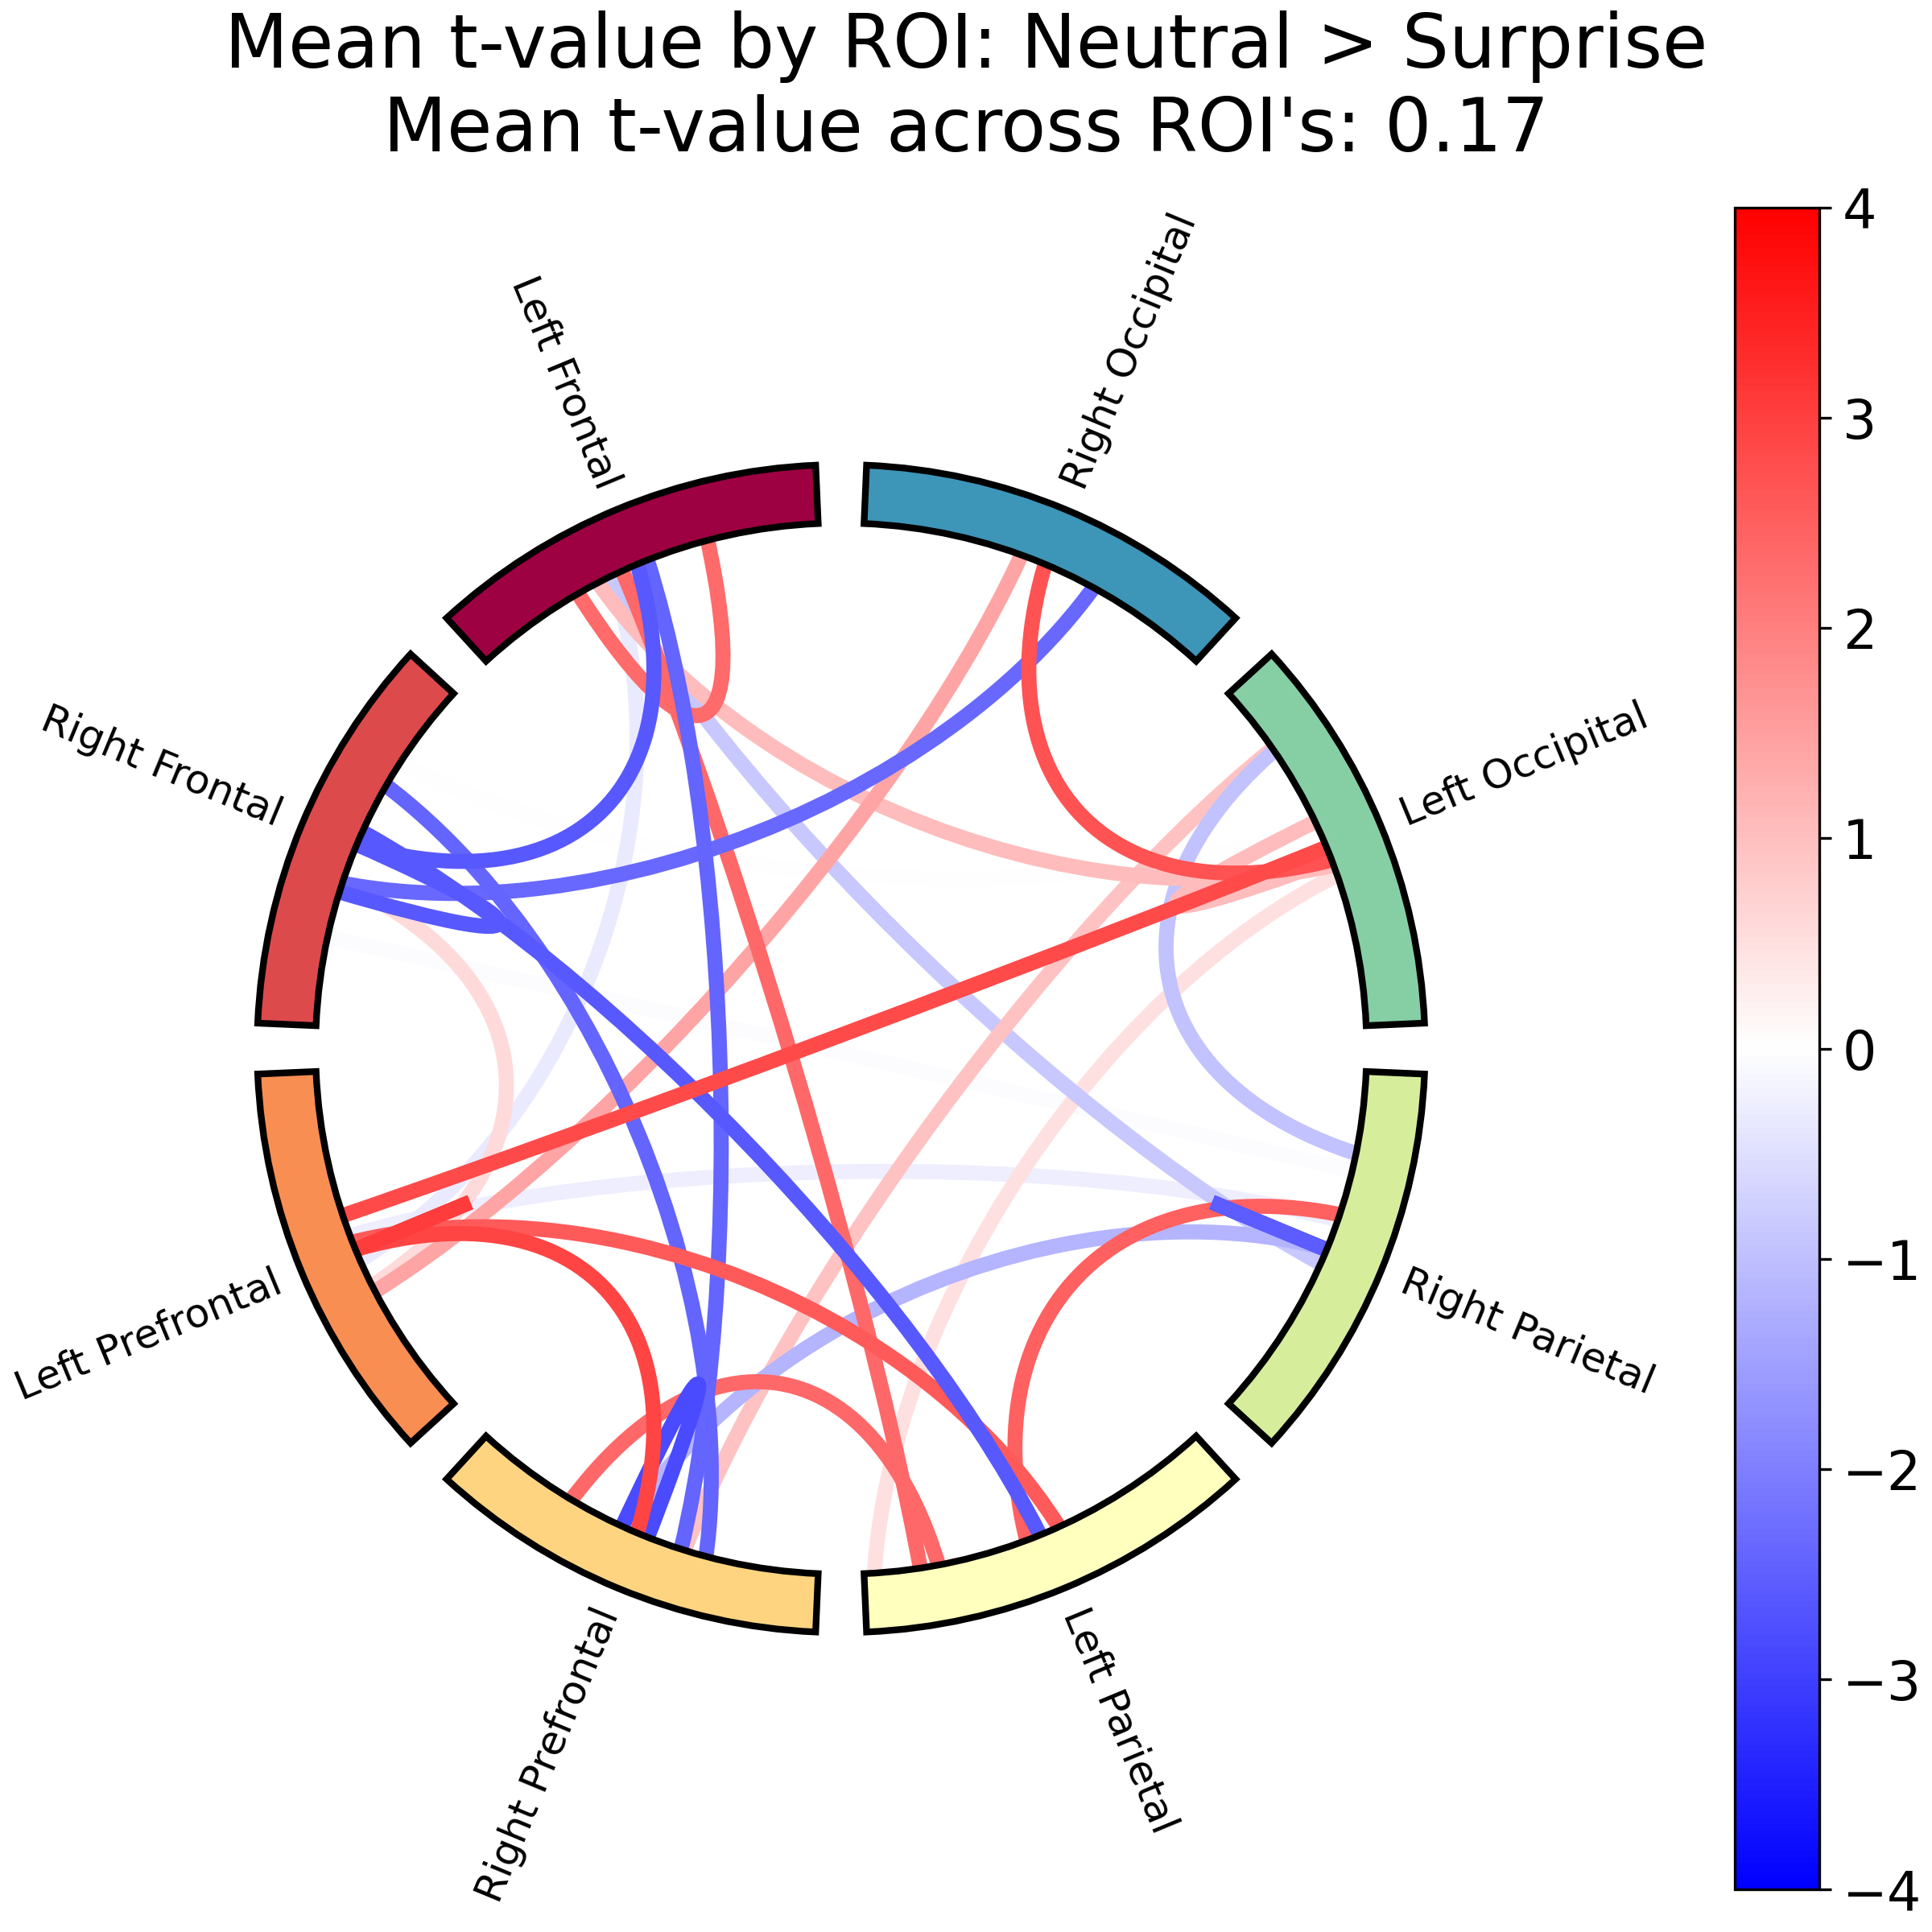
\includegraphics[width=0.49\textwidth]{C:/Users/super/OneDrive - Ontario Tech University/fNIRS_Emotions/plots/spectral_connectivity_time/chord_plots/group_level_t_tests_roi/emotion_Neutral_Surprise.png}
    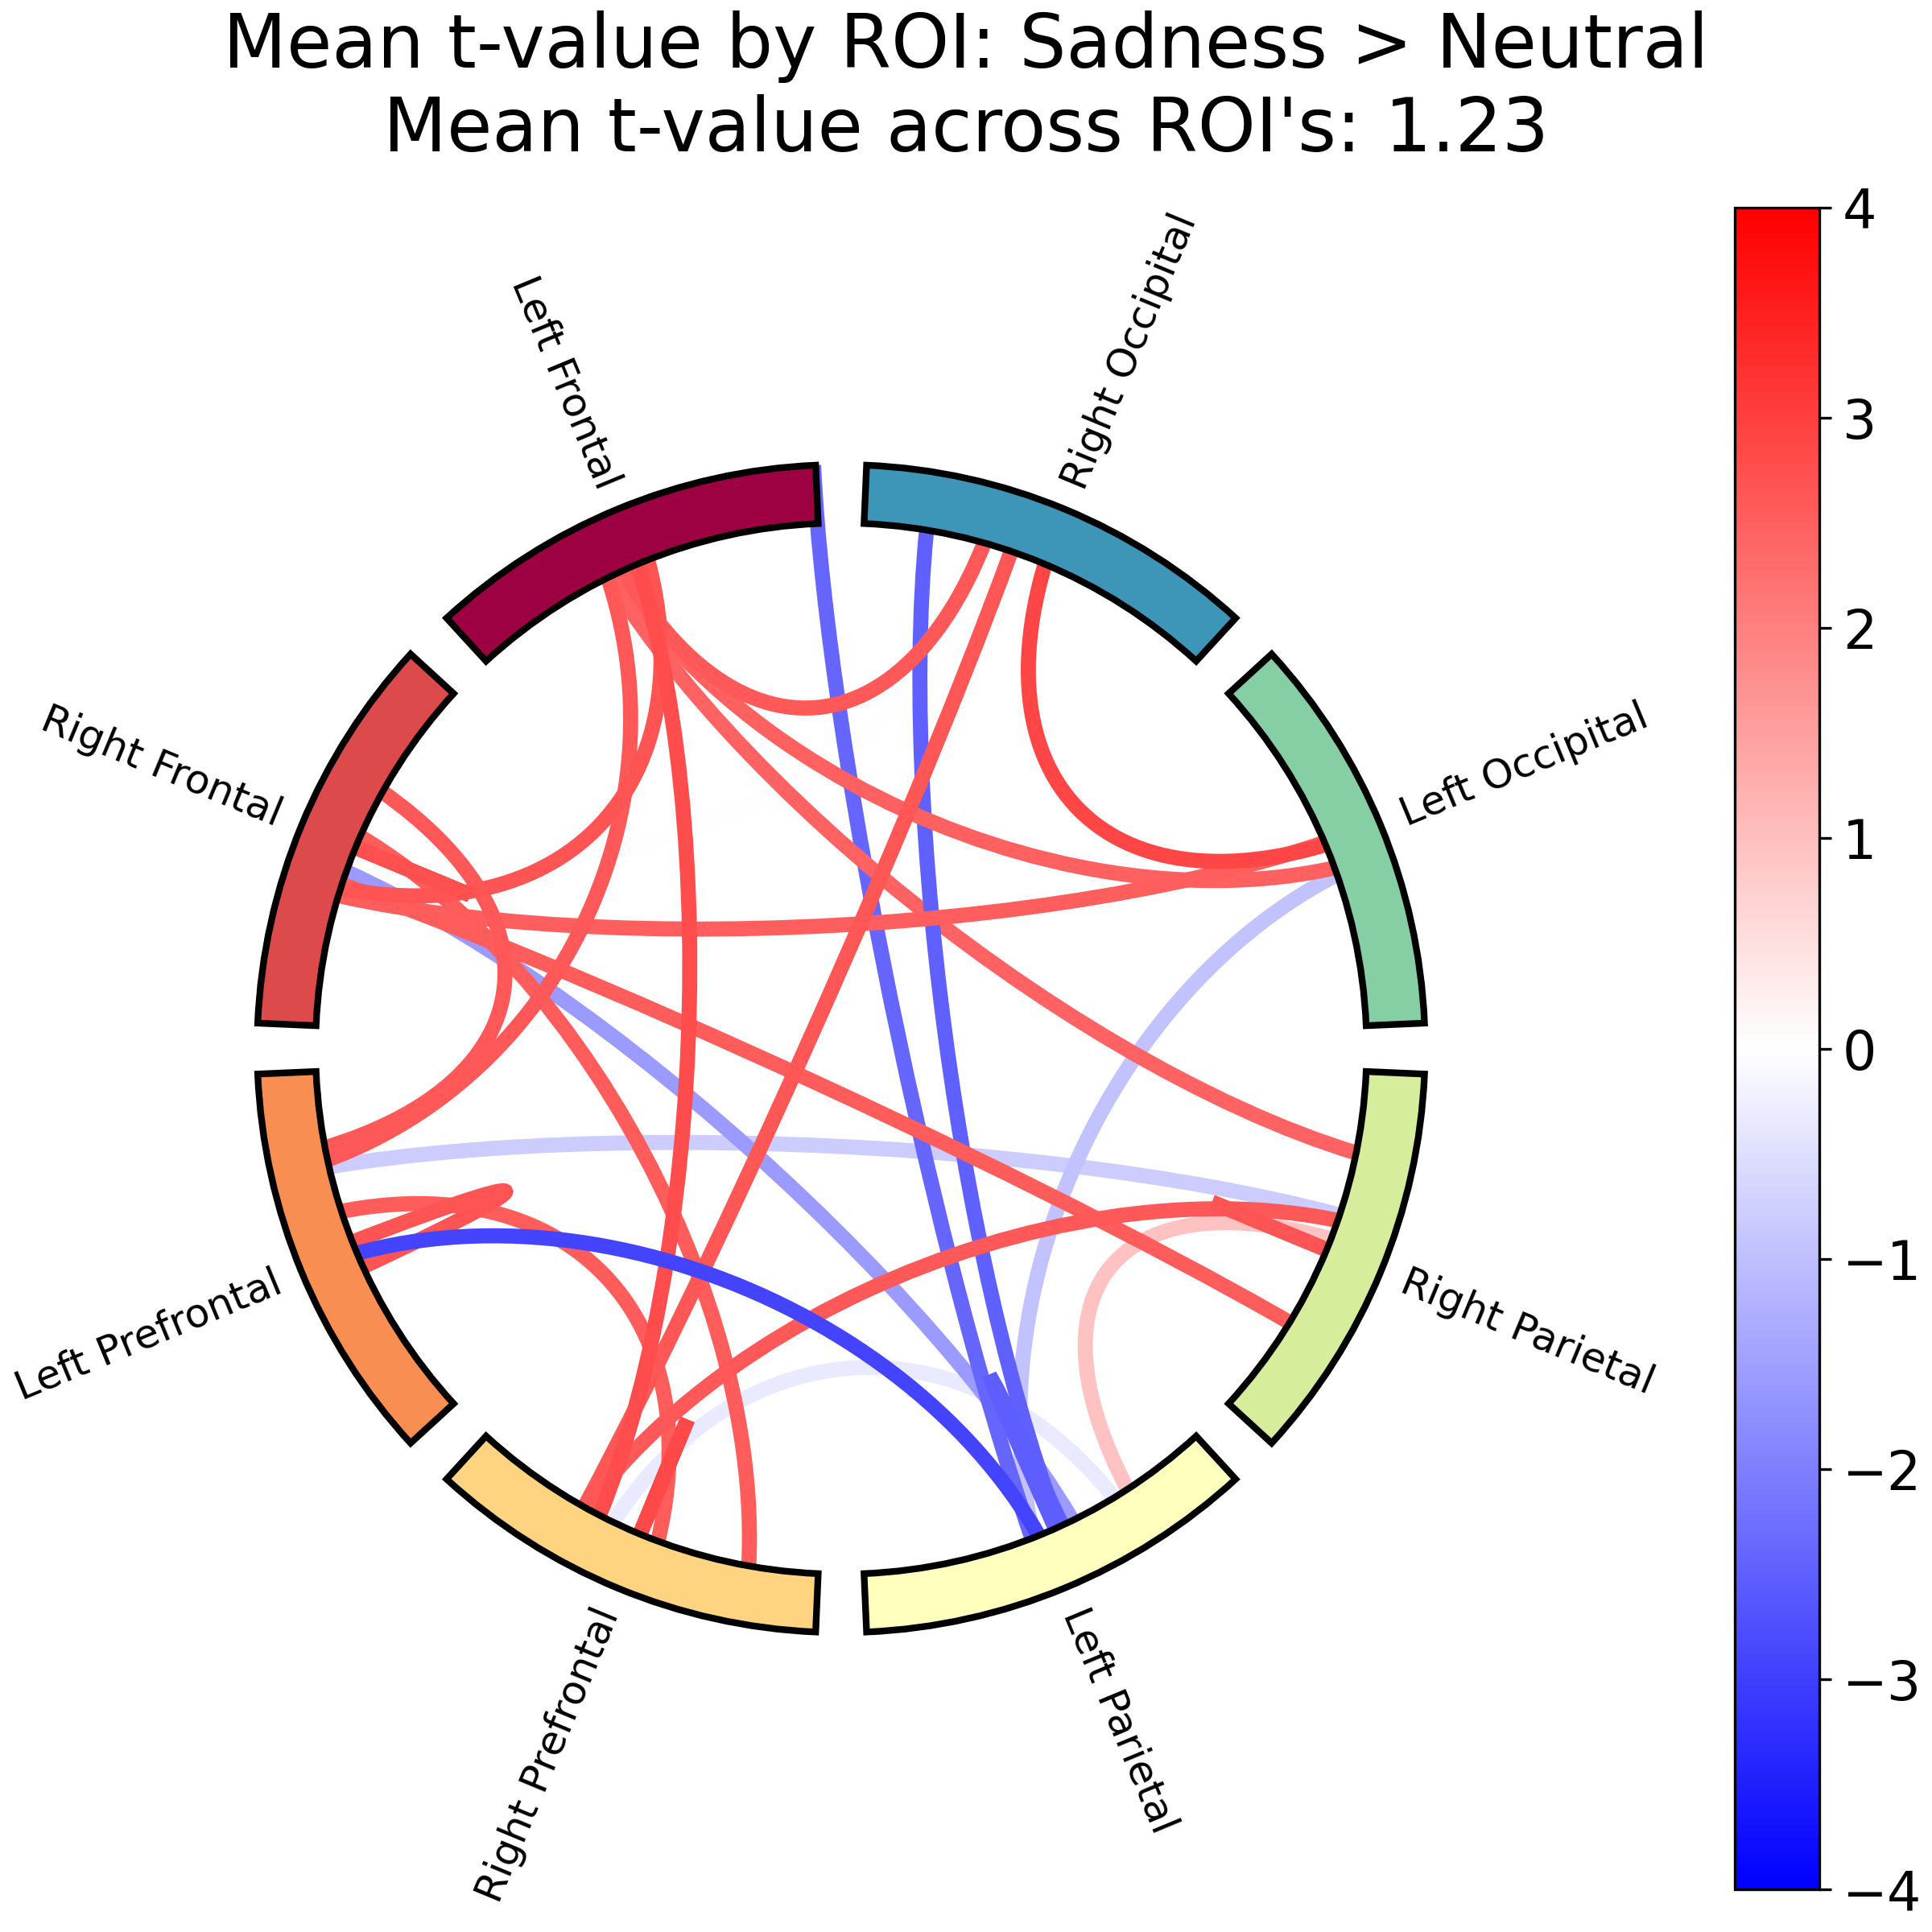
\includegraphics[width=0.49\textwidth]{C:/Users/super/OneDrive - Ontario Tech University/fNIRS_Emotions/plots/spectral_connectivity_time/chord_plots/group_level_t_tests_roi/emotion_Sadness_Neutral.png}
    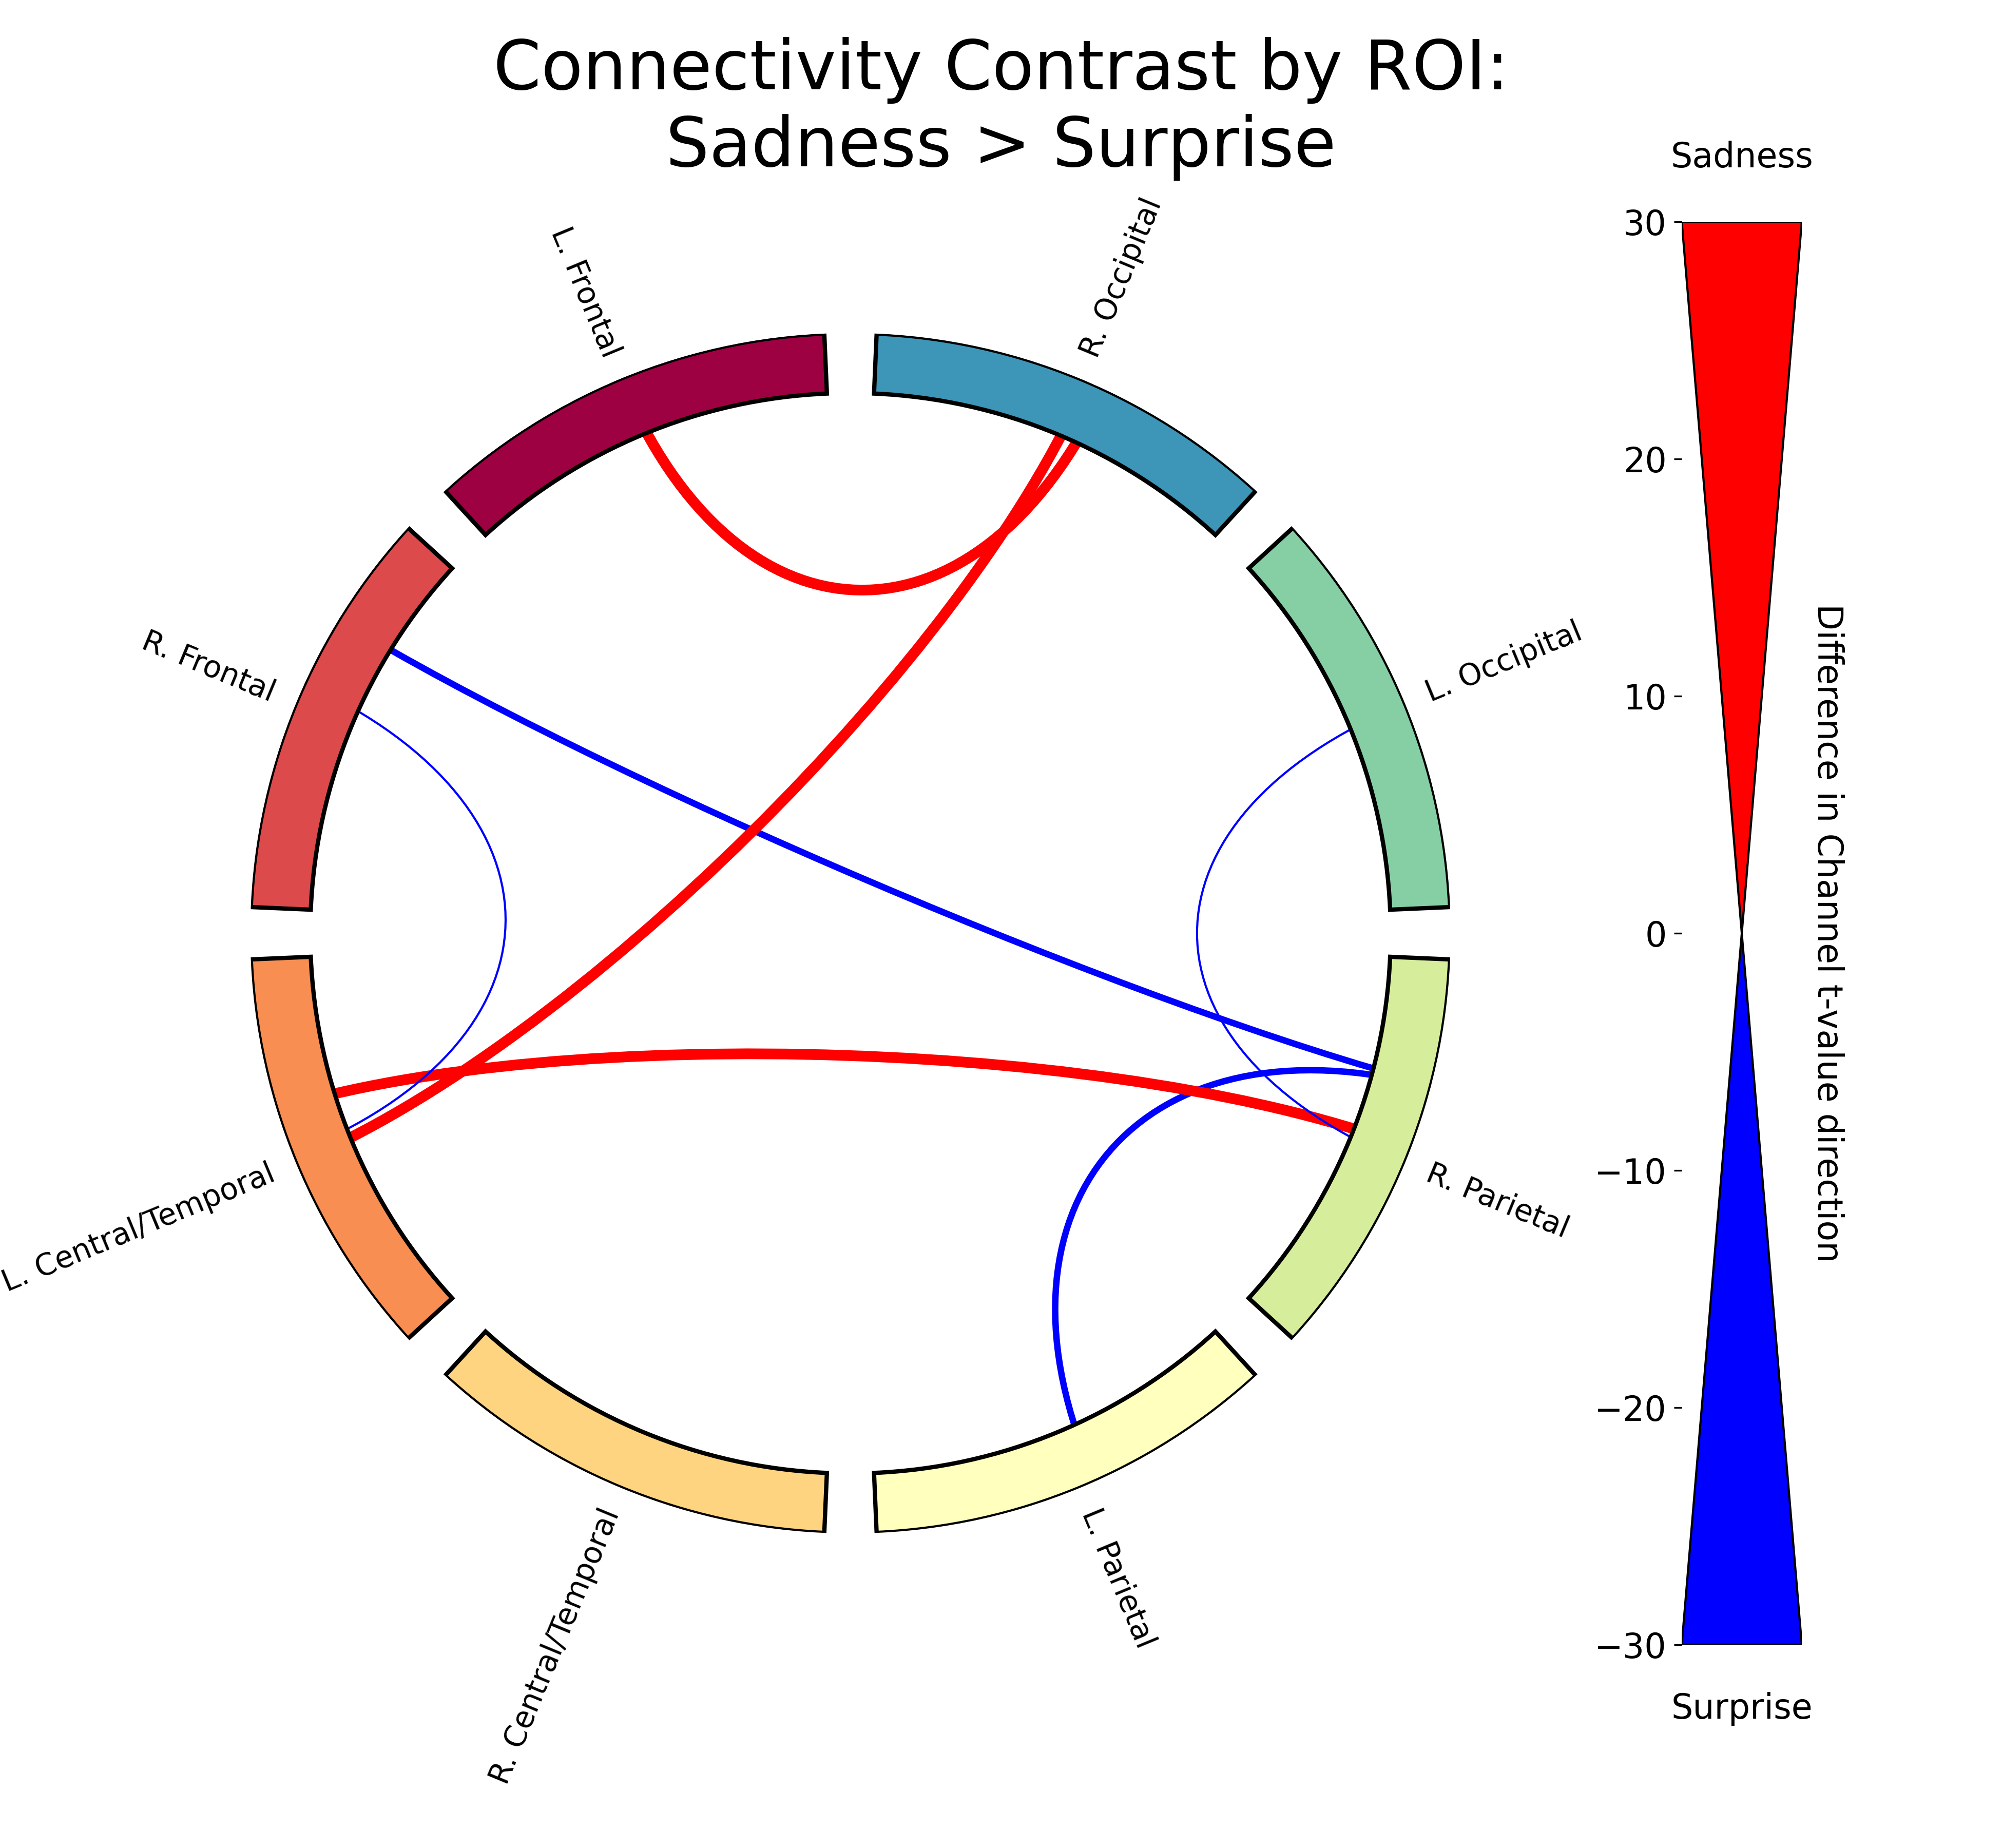
\includegraphics[width=0.49\textwidth]{C:/Users/super/OneDrive - Ontario Tech University/fNIRS_Emotions/plots/spectral_connectivity_time/chord_plots/group_level_t_tests_roi/emotion_Sadness_Surprise.png}
    \caption*{Functional connectivity results for Neutral and Sadness contrasts: Neutral vs. Surprise, Sadness vs. Neutral, and Sadness vs. Surprise. (4/4)}
\end{figure}

\label{tab:appendix_fc_emotion_analysis}
\input{C:/Users/super/OneDrive - Ontario Tech University/fNIRS_Emotions/processed_data/spectral_connectivity_time/group_level_t_tests_roi_contrast_ratios.tex}

\chapter{Memory Task}
\section{ANOVA Results}
\label{tab:appendix_memory_task_anova}
\input{C:/Users/super/OneDrive - Ontario Tech University/fNIRS_Emotions/processed_data/behavioural_responses/anova_table.tex}

\section{Memory Task No Response Distribution}
\begin{figure}[H]
    \centering
    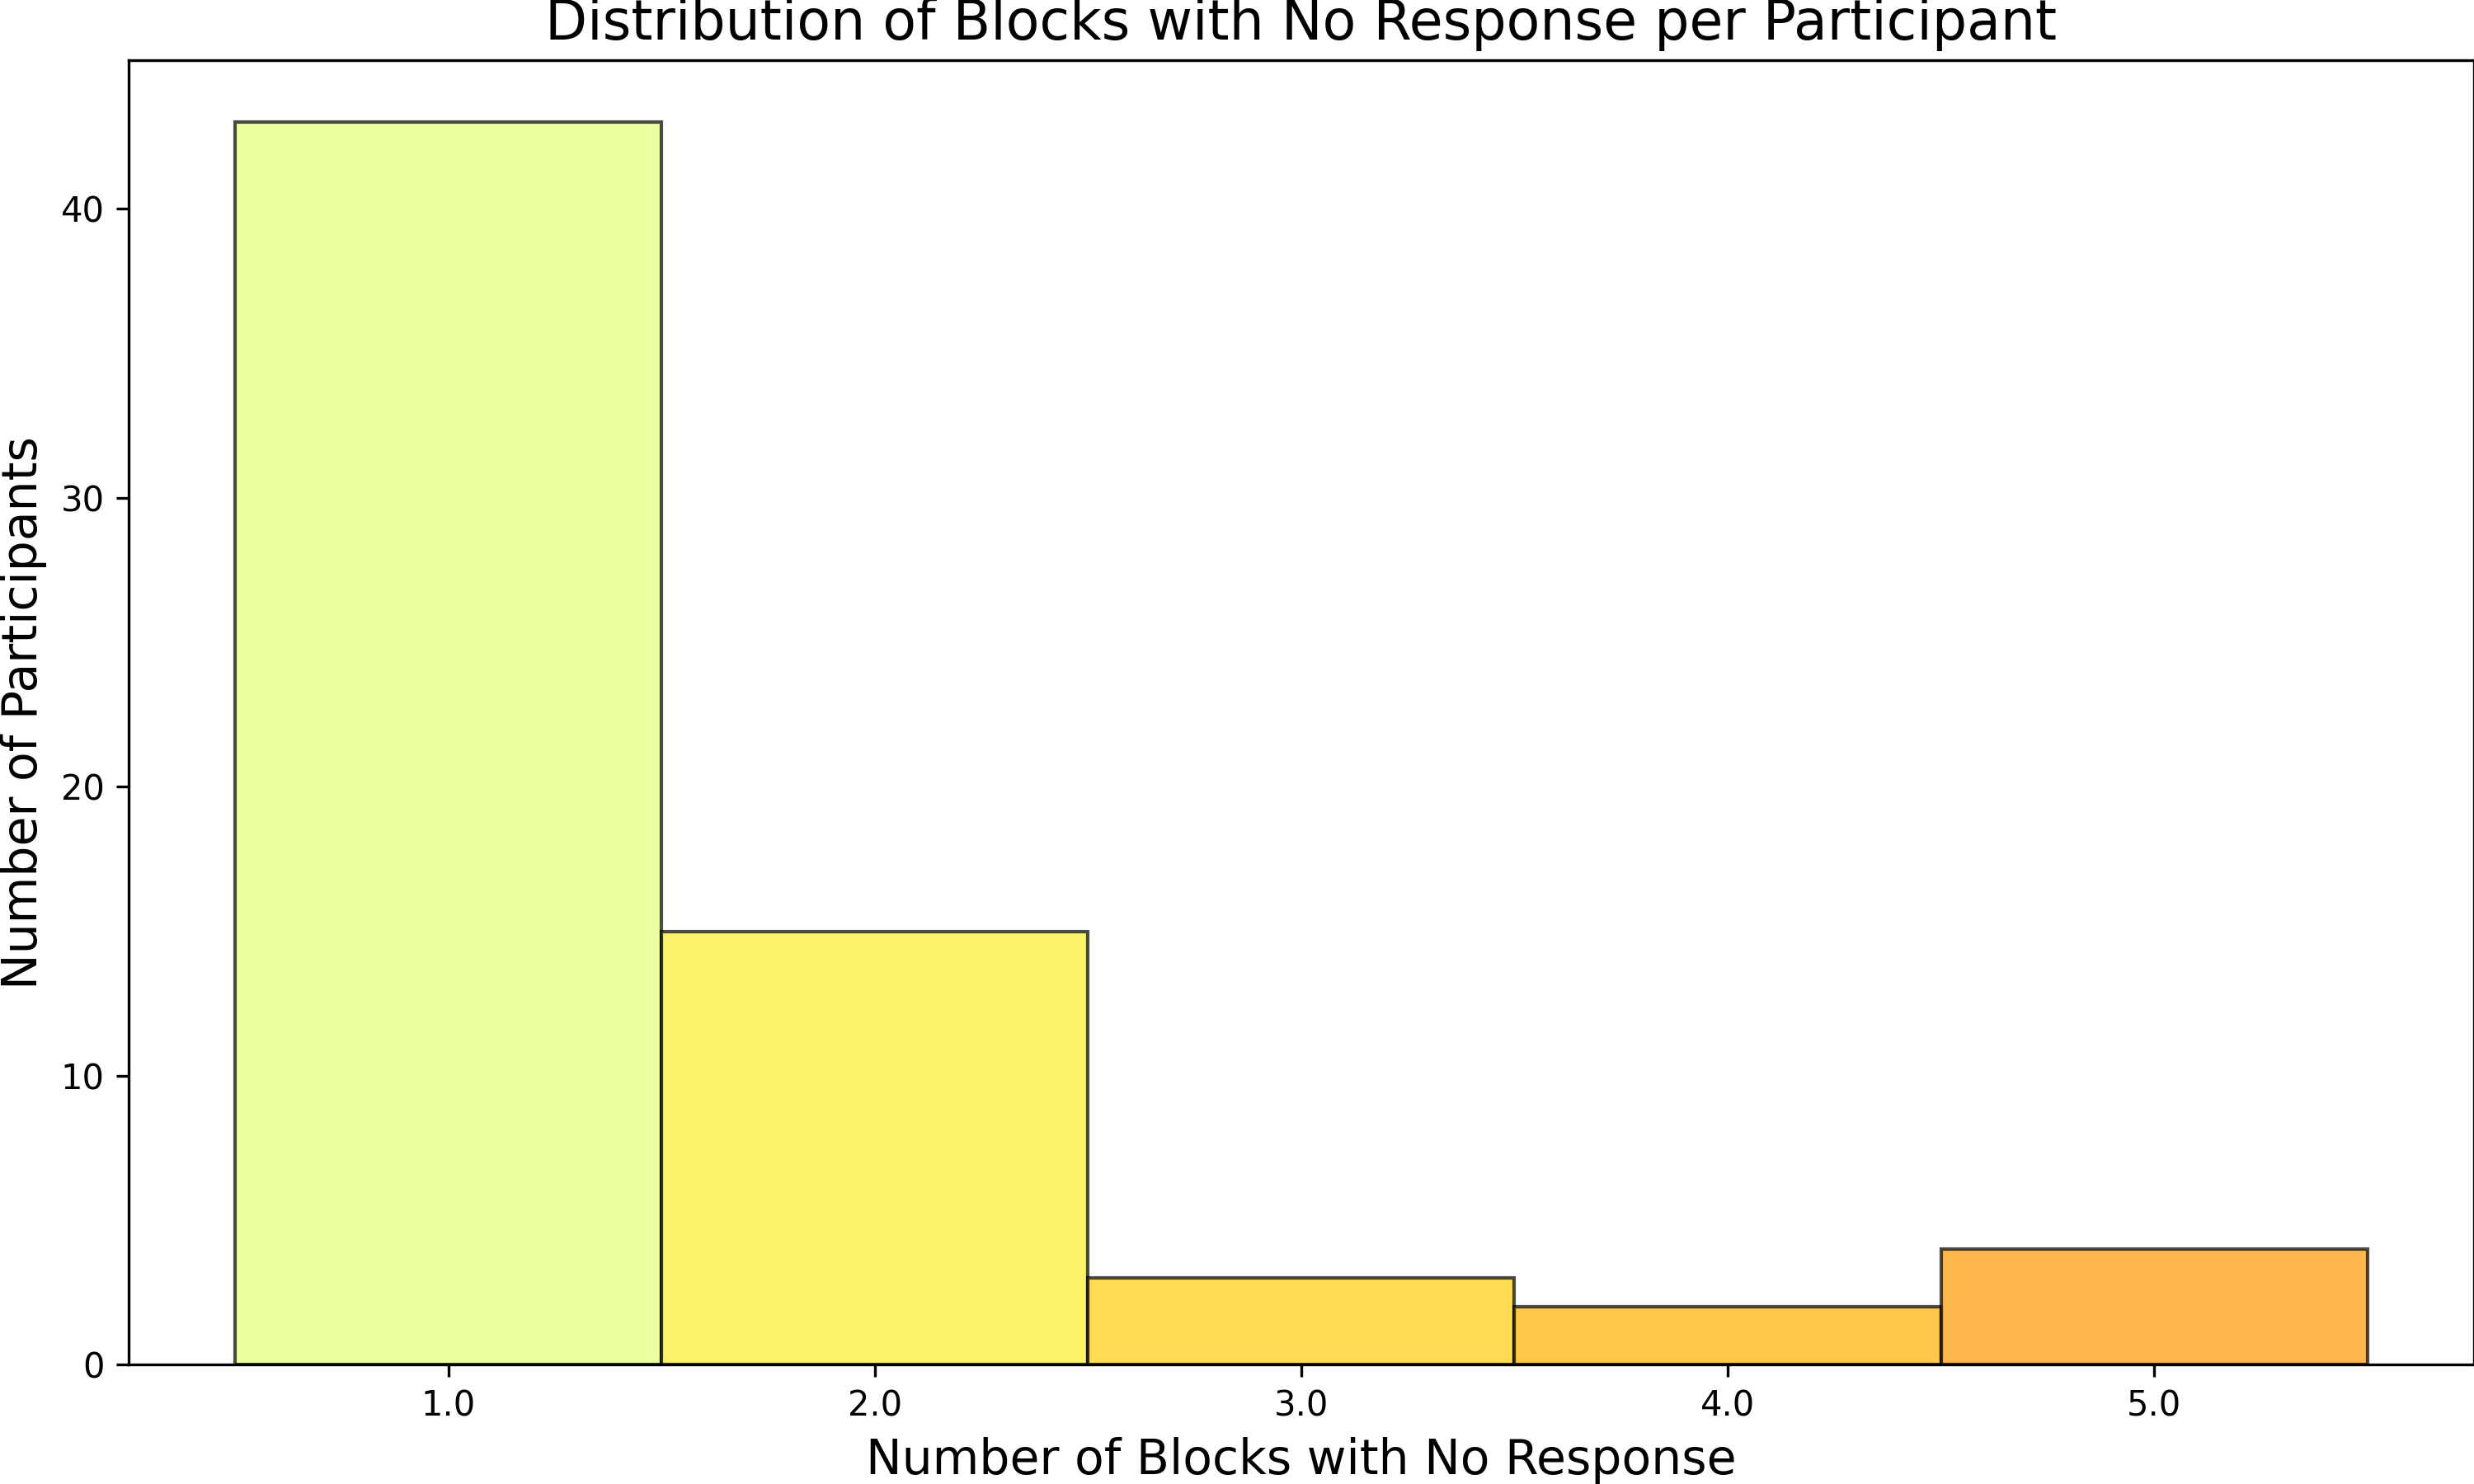
\includegraphics[width=1\textwidth]{C:/Users/super/OneDrive - Ontario Tech University/fNIRS_Emotions/plots/behavioural_responses/no_response_counts.png}
    \caption[Memory Task No Response Distribution]{Distribution of the number of no responses across the 56 blocks for each participant in the memory task.}
    \label{fig:appendix_memory_task_no_response_distribution}
\end{figure}